Tout comme pour les quadrilatères, la convexité va jouer un rôle central pour l’isopérimétrie polygonale dans le cas général
%
Ceci explique que nous allons chercher à justifier l'existence d'au moins un \ngone\ convexe d'aire maximale parmi les \ngones\ convexes de longueur fixée.


% ----------------------- %


\begin{fact} \label{conv-pos-det}
    Pour tout \ngone\ convexe $\setproba{P} = A_1 A_2 \cdots A_n$, l'une des alternatives suivantes a lieu.
    %
	\begin{itemize}
		\item $\forall (i, k) \in \ZintervalC{1}{n}^2$,
		si $k \notin \setgene{i ; i+1}$, alors
		$\det \big( \vect{\primeit{A}_i \primeit{A}_{i+1}}, \vect{\primeit{A}_i \primeit{A}_k} \big) > 0$.

		\item $\forall (i, k) \in \ZintervalC{1}{n}^2$,
		si $k \notin \setgene{i ; i+1}$, alors
		$\det \big( \vect{\primeit{A}_i \primeit{A}_{i+1}}, \vect{\primeit{A}_i \primeit{A}_k} \big) < 0$.
    \end{itemize}
\end{fact}


\begin{proof}
	Le cas $n = 3$ des triangles est immédiat.
	Considérons alors $\setproba{P}$ un \ngone\ convexe où  $n \geq 4$.
	Nous savons que, relativement à $\setproba{P}$, aucun triplet de sommets consécutifs alignés n'existe.
	Dès lors, dans le plan orienté, les trois premiers sommets sont placés suivant l'une des deux configurations suivantes. 
    
    \begin{multicols}{2}
        \small\itshape\centering
       	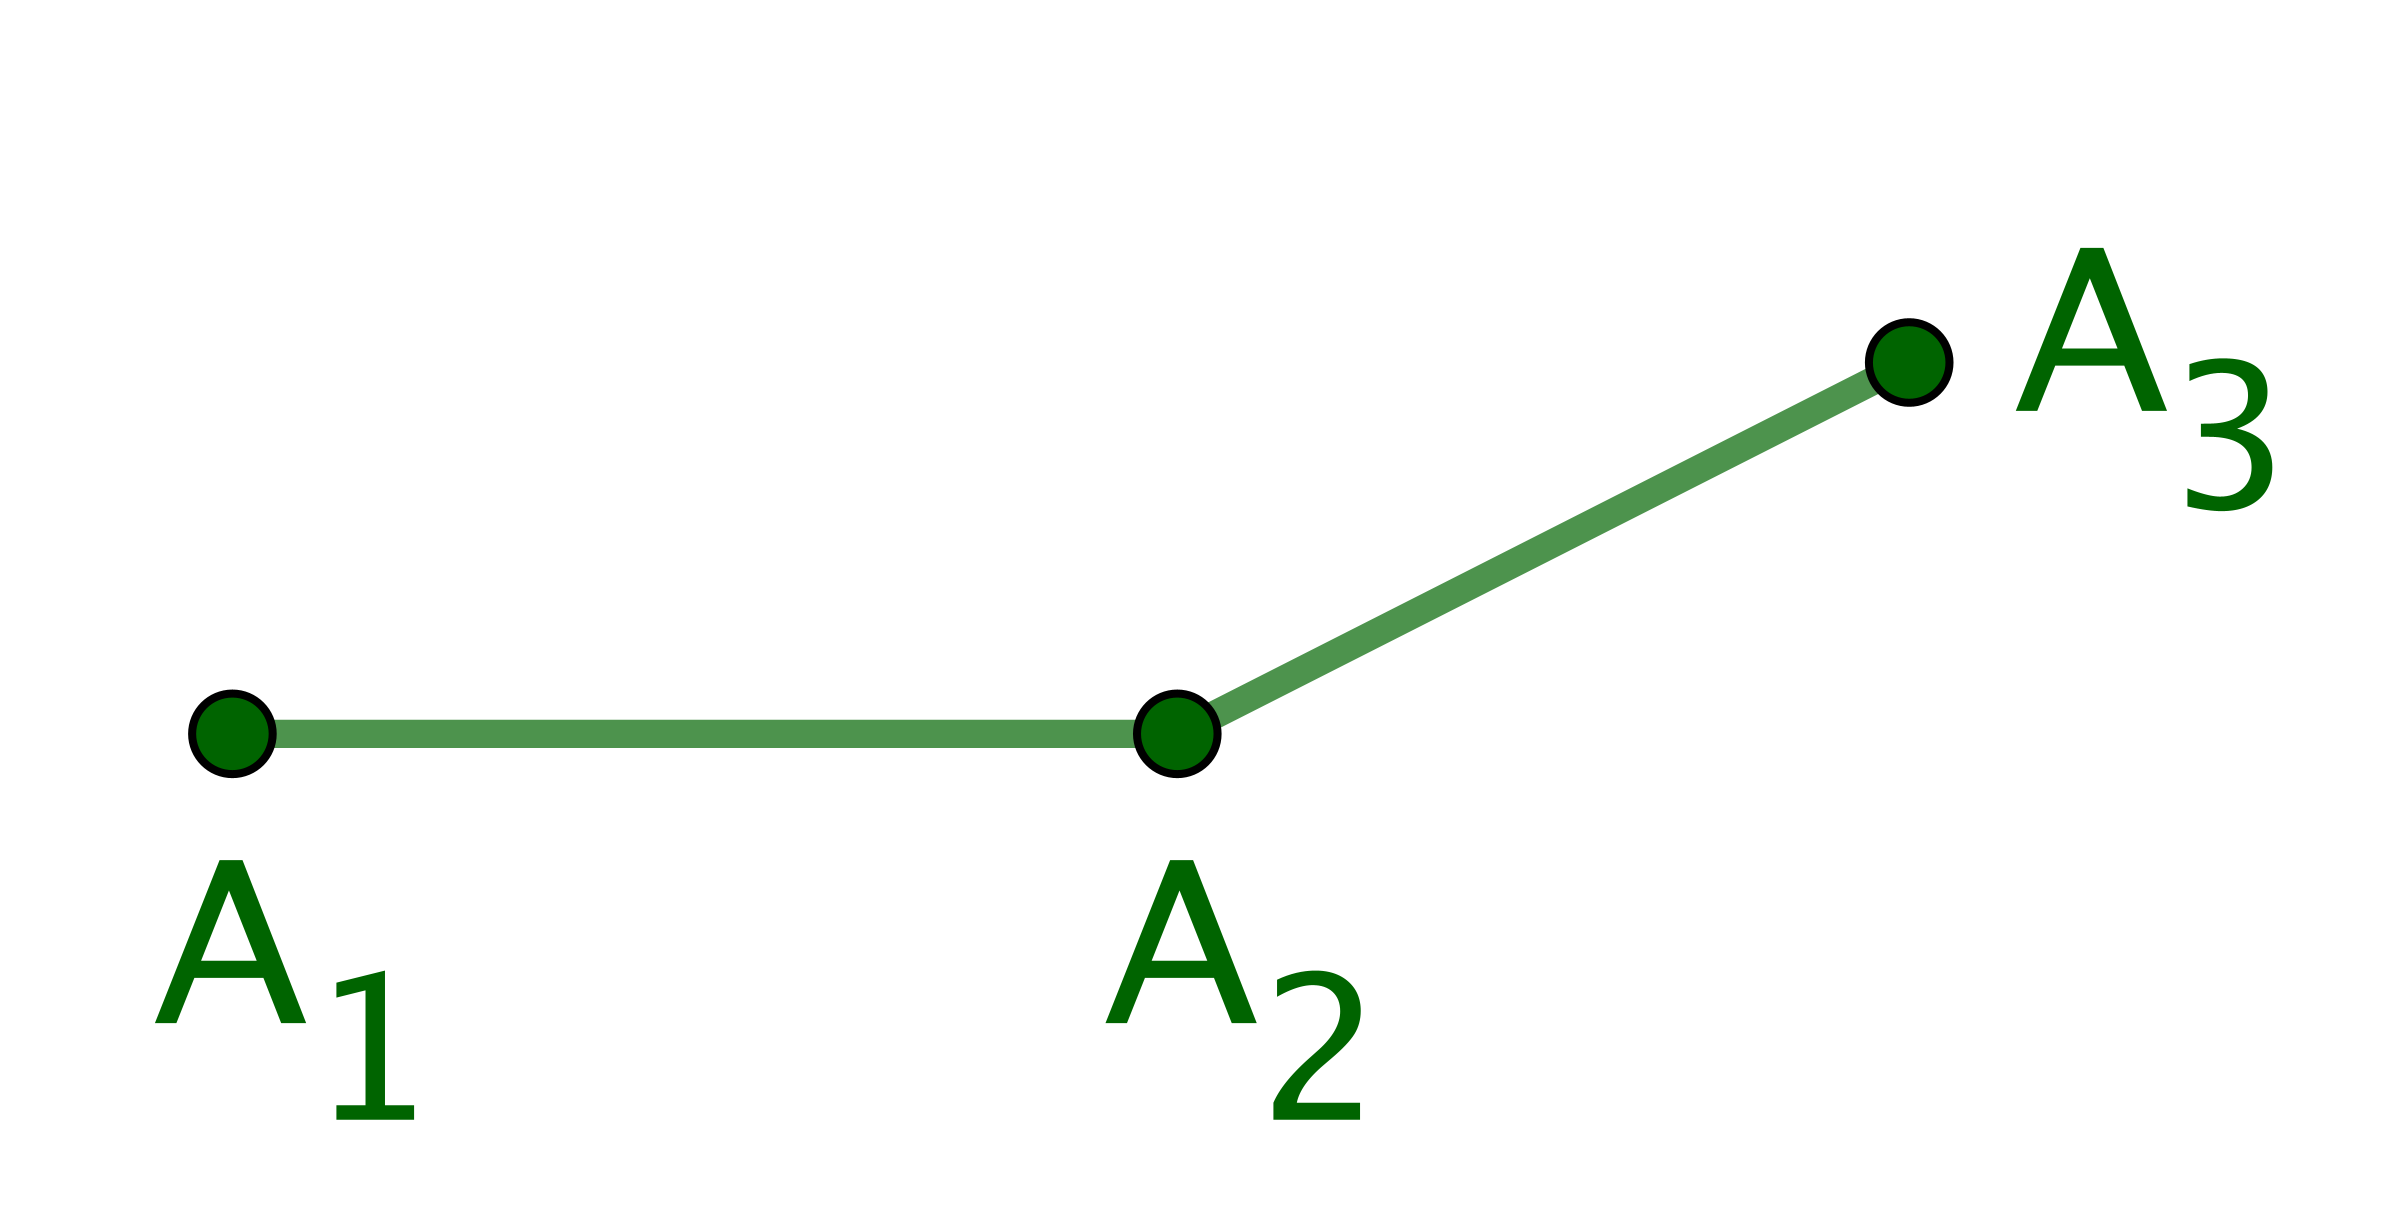
\includegraphics[scale=.45]{content/polygon/at-least-one/conv-det-sign-1.png}
    	    
    	\smallskip
        Cas positif.
        
        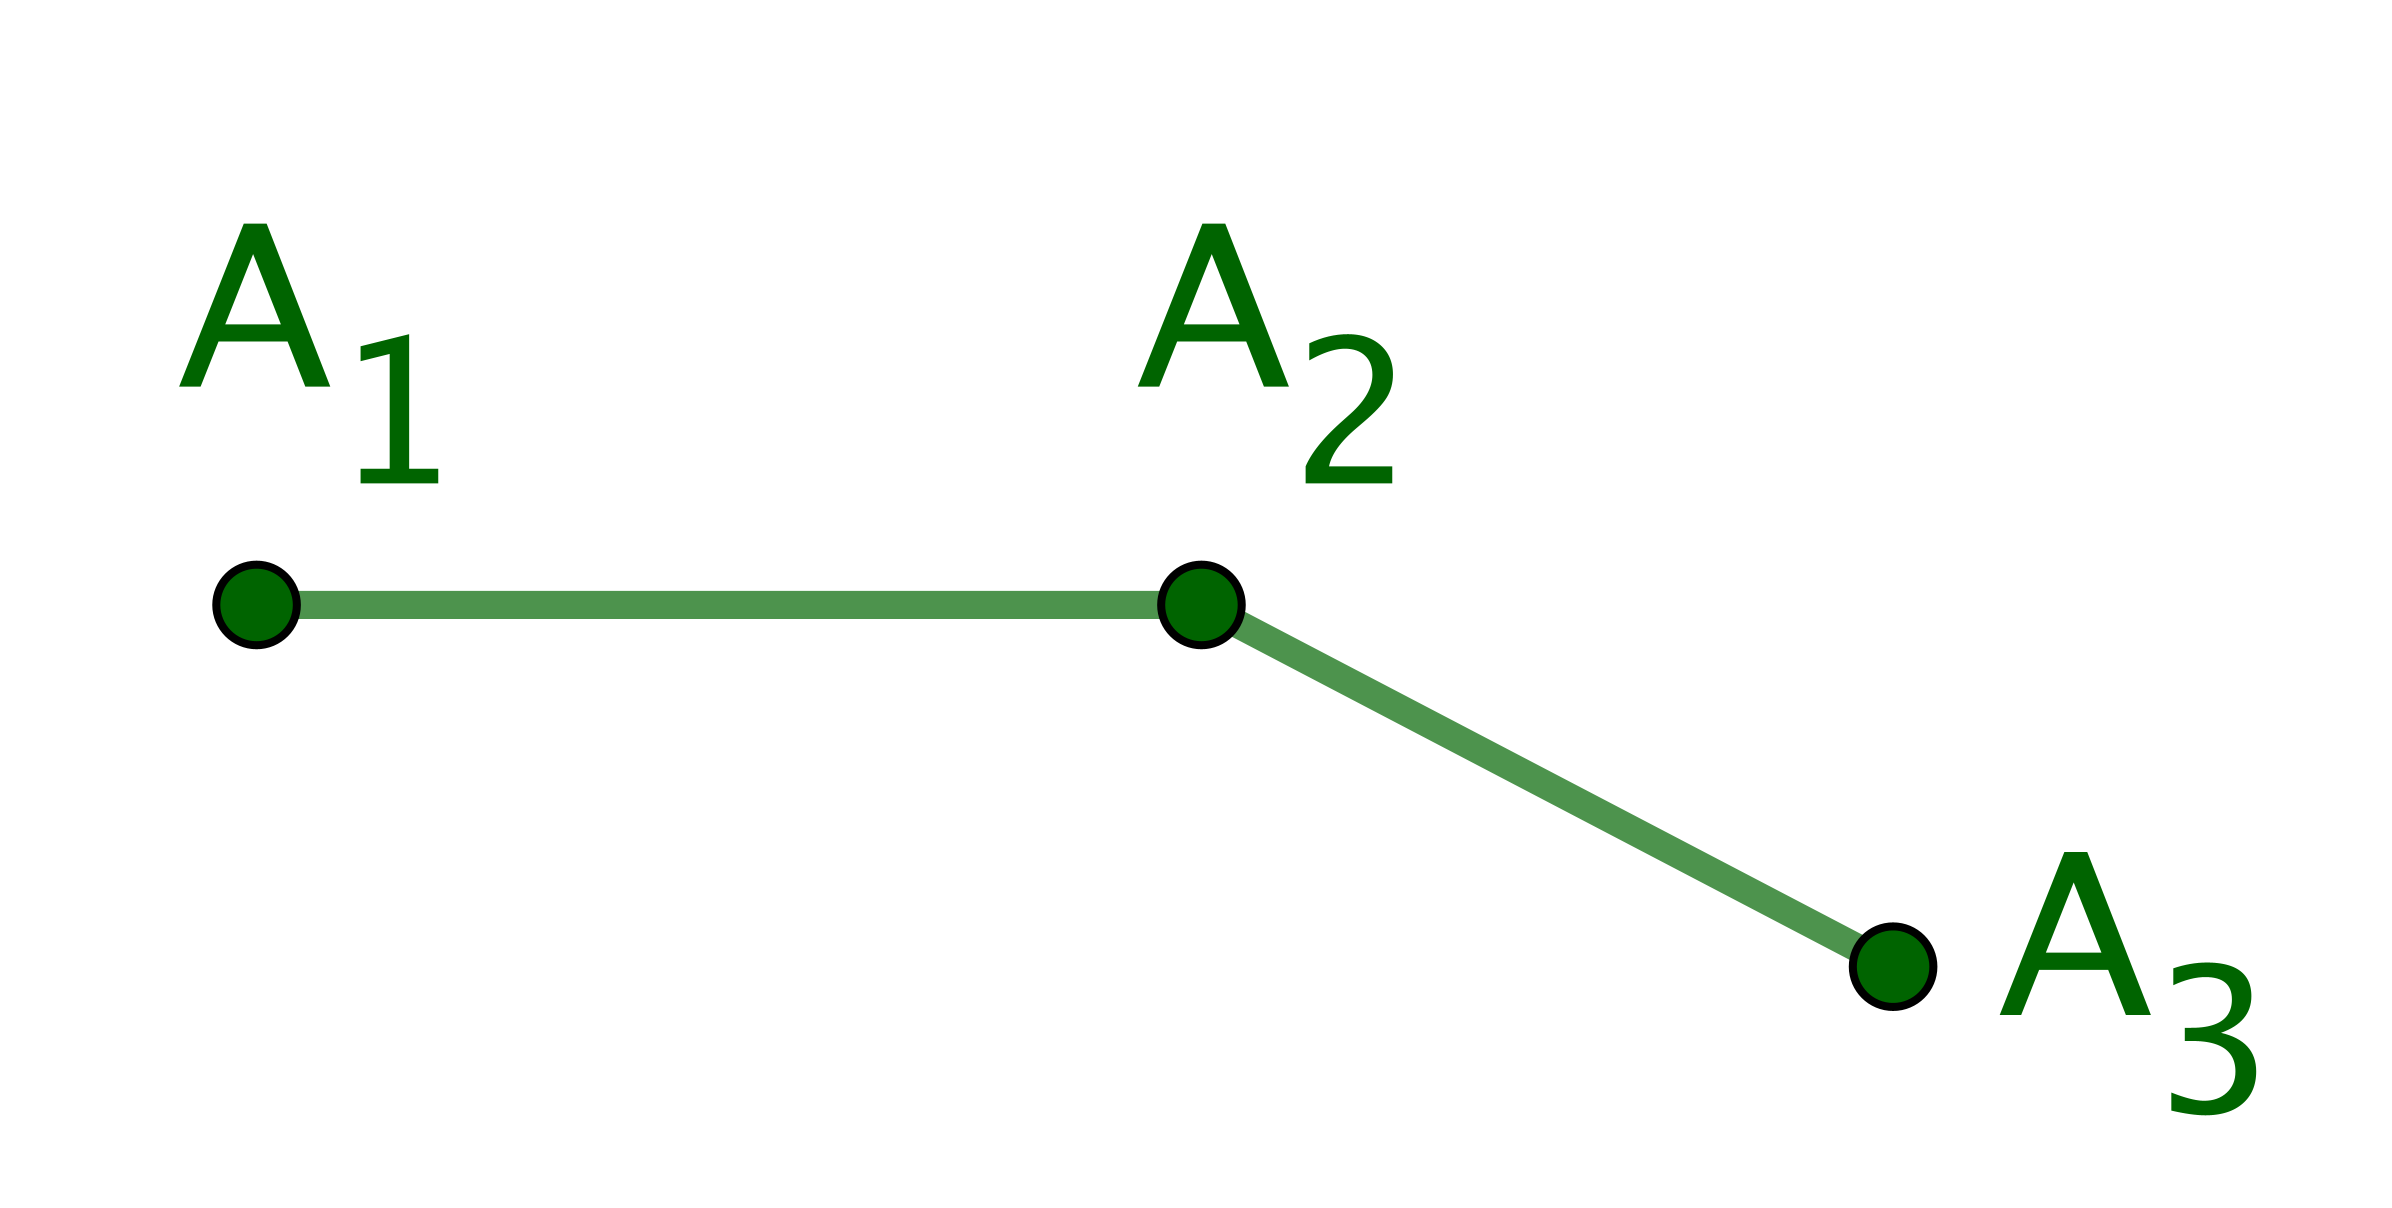
\includegraphics[scale=.45]{content/polygon/at-least-one/conv-det-sign-2.png}
    	    
    	\smallskip
        Cas négatif.
    \end{multicols}

    
    \newpage


    \noindent
    Considérons le cas positif, c'est-à-dire supposons que 
    $\det \big( \vect{\primeit{A}_1 \primeit{A}_2}, \vect{\primeit{A}_1 \primeit{A}_3} \big) > 0$.
	%
	\begin{itemize}
    	\item $\vect{\primeit{A}_1 \primeit{A}_3} = \vect{\primeit{A}_1 \primeit{A}_2} + \vect{\primeit{A}_2 \primeit{A}_3}$
    	donne
		$\det \big( \vect{\primeit{A}_2 \primeit{A}_3}, \vect{\primeit{A}_2 \primeit{A}_1} \big) > 0$.


		\item Comme $A_2$, $A_3$ et $A_4$ ne sont pas alignés, et de plus $A_1$ et $A_4$ du même côté de la droite $(A_2 A_3)$, au sens large, nous obtenons
		$\det \big( \vect{\primeit{A}_2 \primeit{A}_3}, \vect{\primeit{A}_2 \primeit{A}_4} \big) > 0$.


		\item En continuant de proche en proche, nous arrivons à
		$\det \big( \vect{\primeit{A}_i \primeit{A}_{i+1}}, \vect{\primeit{A}_i \primeit{A}_{i+2}} \big) > 0$
		pour $i \in \ZintervalC{1}{n}$ quelconque.


		\item Le point précédent et la convexité donnent
		$\det \big( \vect{\primeit{A}_i \primeit{A}_{i+1}}, \vect{\primeit{A}_i \primeit{A}_k} \big) \geq 0$
		pour $(i, k) \in \ZintervalC{1}{n}^2$ tel que $k \notin \setgene{i ; i+1}$.


		\item
		Montrons maintenant que
		$\det \big( \vect{\primeit{A}_1 \primeit{A}_2}, \vect{\primeit{A}_1 \primeit{A}_k} \big) > 0$
		pour $k \in \ZintervalC{3}{n}$.
		%
		Nous savons déjà l'inégalité vraie pour $k = 3$; passons donc à $k = 4$.
		Pour avoir 
		$\det \big( \vect{\primeit{A}_1 \primeit{A}_2}, \vect{\primeit{A}_1 \primeit{A}_4} \big) > 0$, 
		le point précédent donne qu'il faut vérifier que 
		$\det \big( \vect{\primeit{A}_1 \primeit{A}_2}, \vect{\primeit{A}_1 \primeit{A}_4} \big) = 0$
		est impossible.
		Supposons donc l'égalité vraie, ce qui implique d'avoir $n \geq 5$, car dans le cas contraire les sommets consécutifs $A_4$, $A_1$ et $A_2$ seraient alignés.
		Nous aboutissons aux configurations suivantes où les hachures et la droite en trait plein sont des zones interdites pour $A_4$.

        \begin{multicols}{2}
            \small\itshape\centering
           	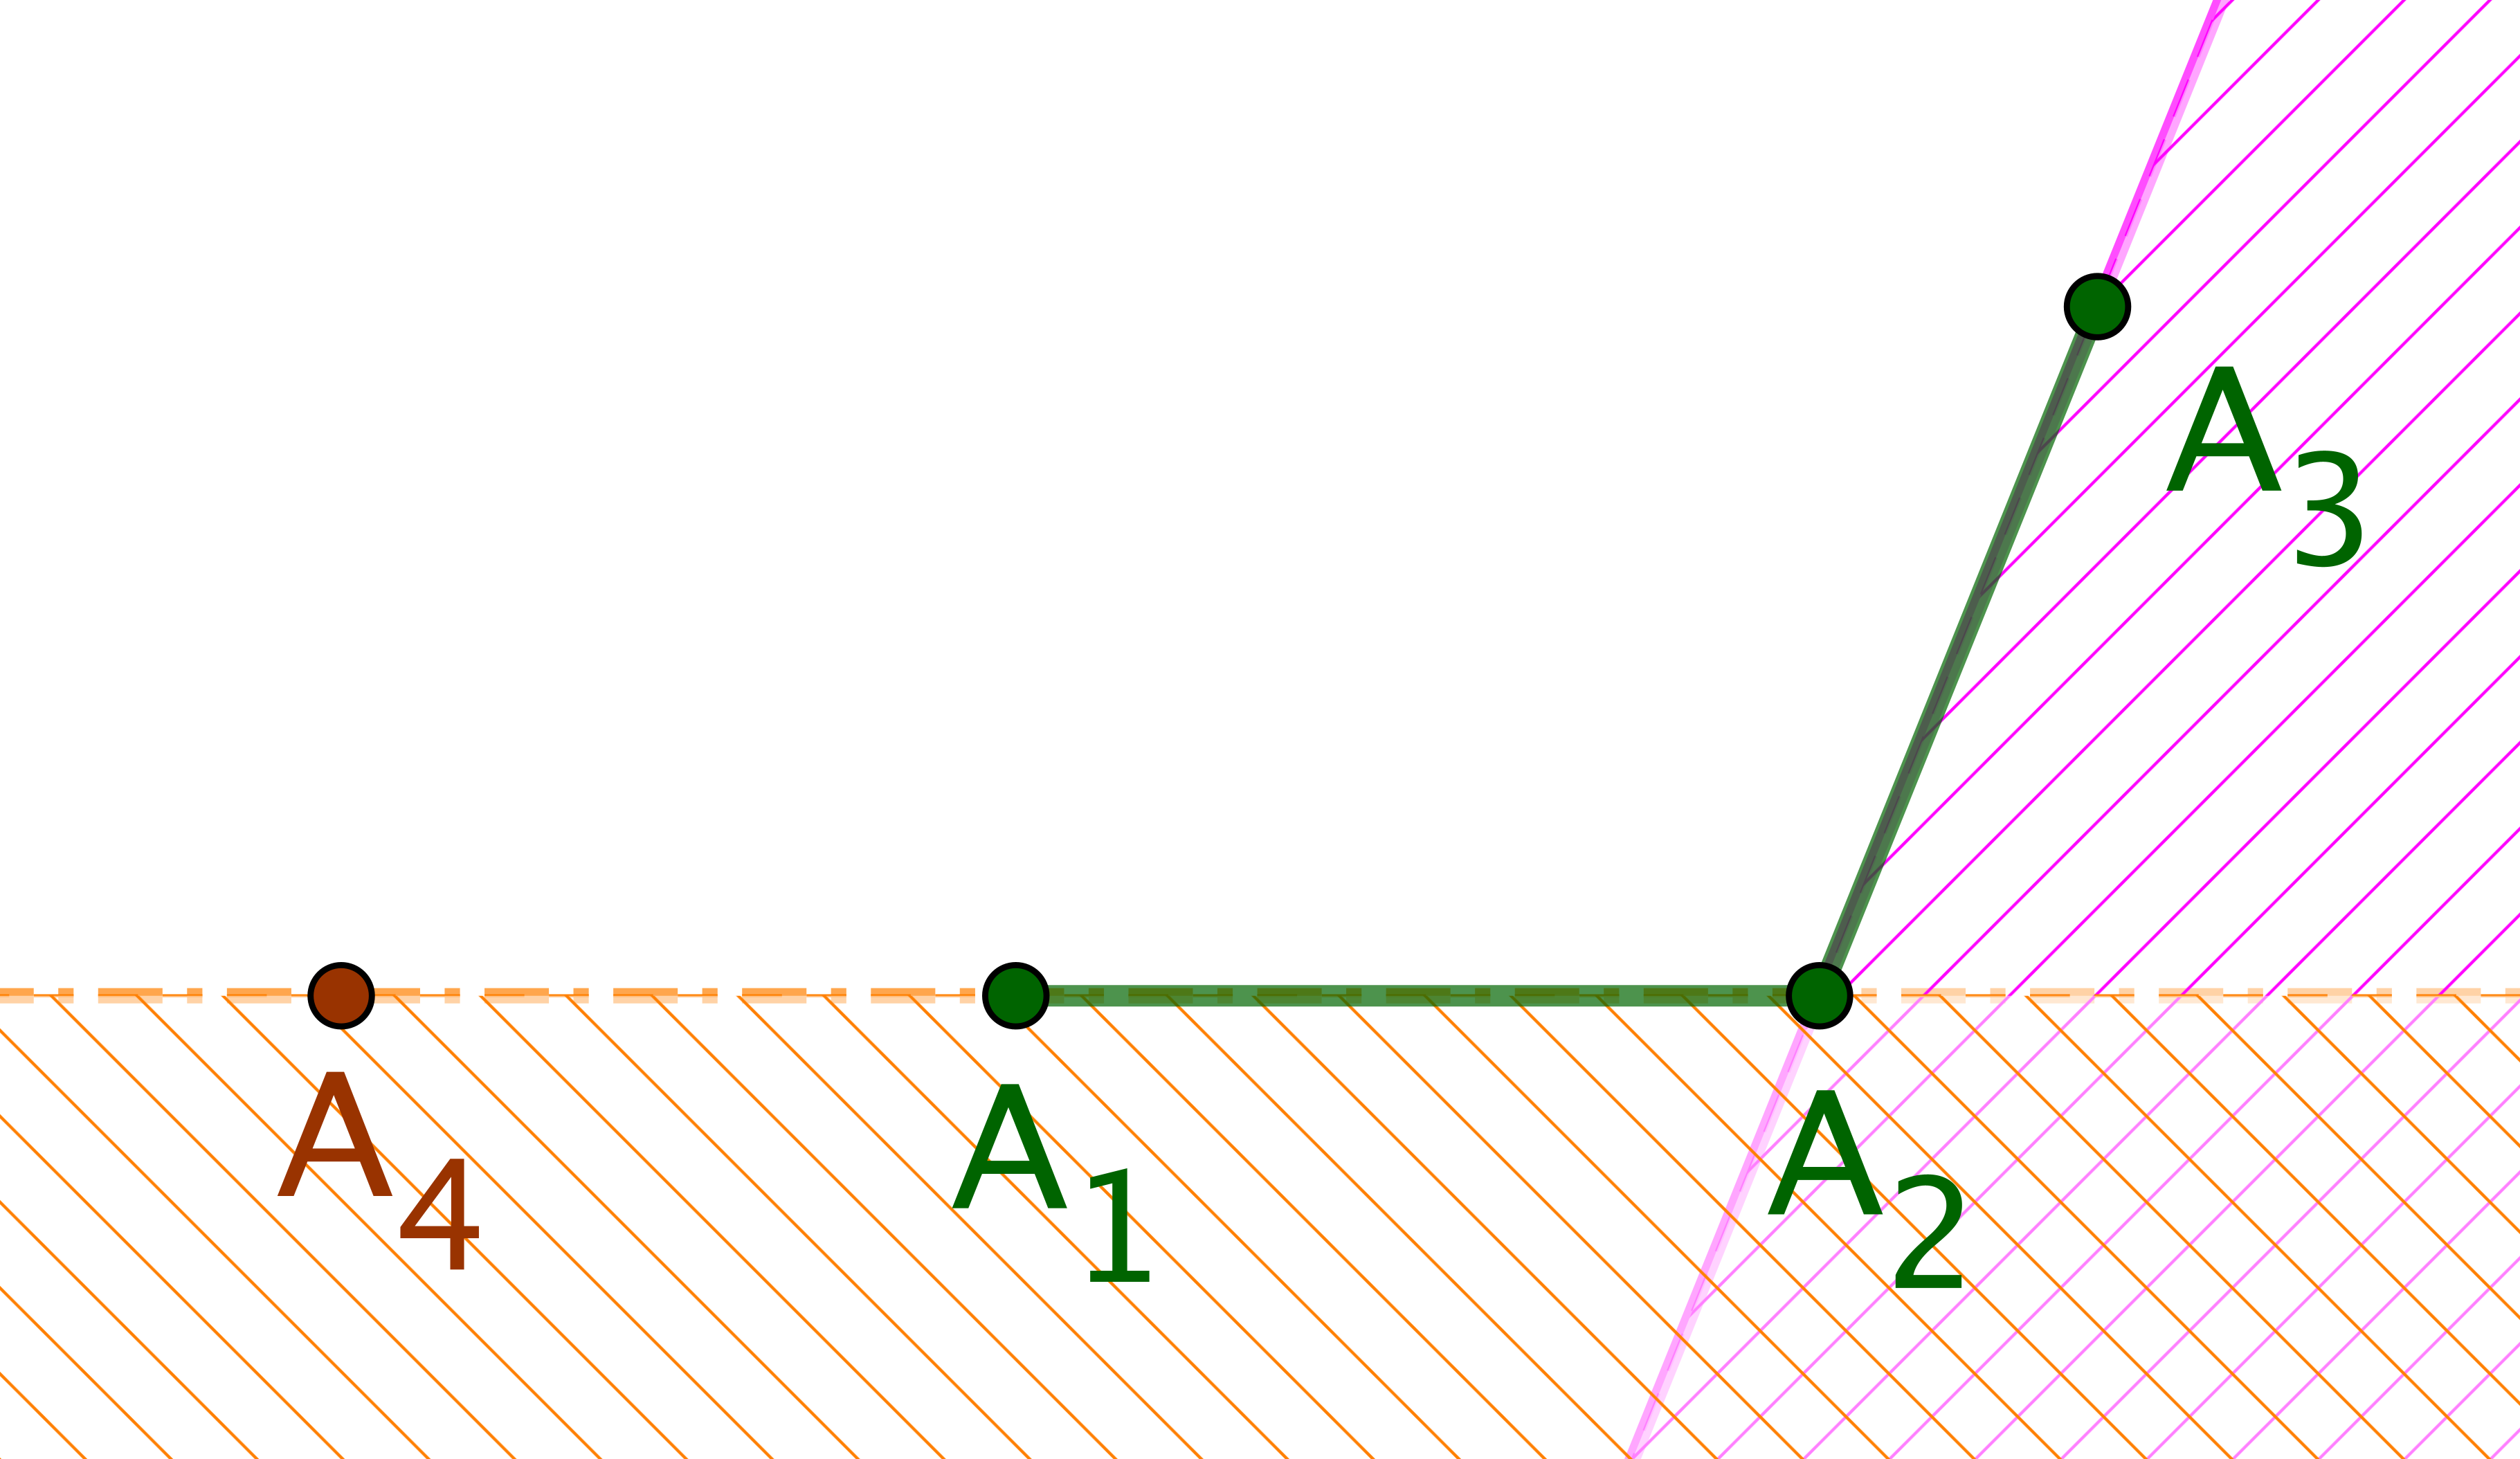
\includegraphics[scale=.4]{content/polygon/at-least-one/conv-det-A4-1.png}
        	    
        	\smallskip
            Cas 1.
            
            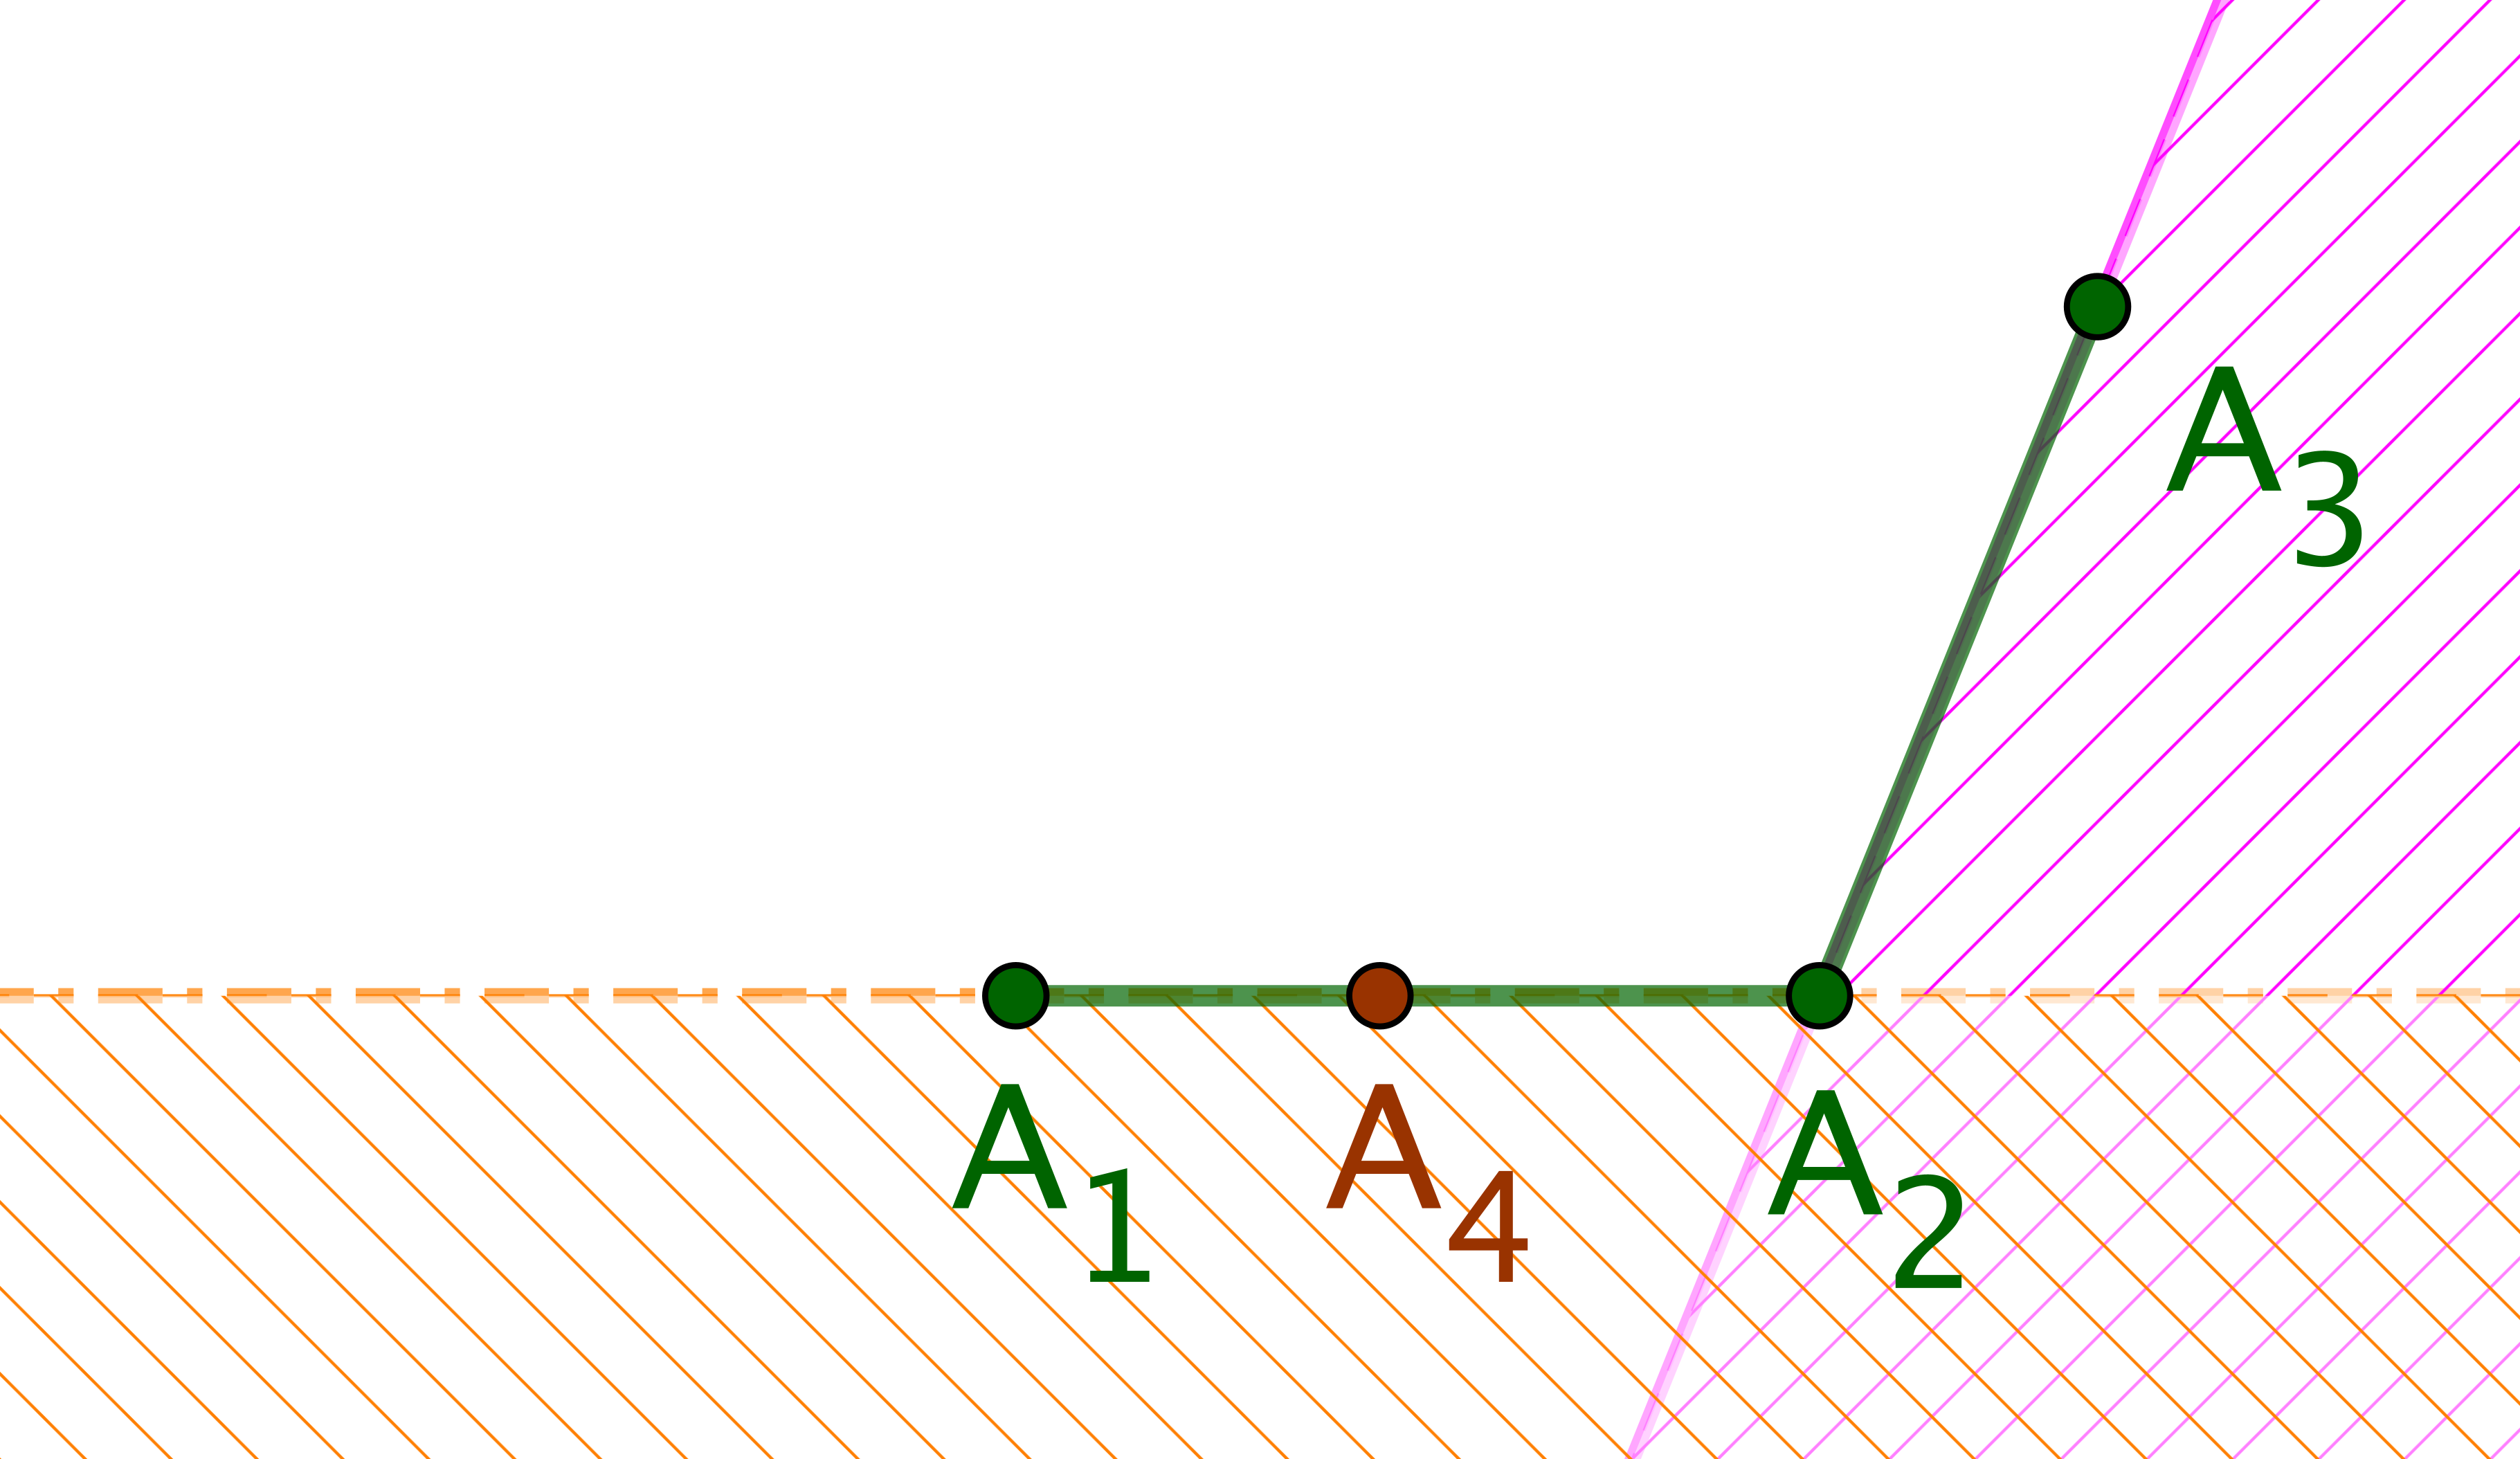
\includegraphics[scale=.4]{content/polygon/at-least-one/conv-det-A4-2.png}
        	    
        	\smallskip
            Cas 2.
        \end{multicols}
    
		\noindent
		Le cas 2 est impossible par raison de convexité, car $A_1$ et $A_2$ sont de part et d'autre de la droite $(A_3 A_4)$. Voyons donc ce qu'implique le 1\ier\ cas pour $A_5$.
		
        \begin{multicols}{2}
            \small\itshape\centering
           	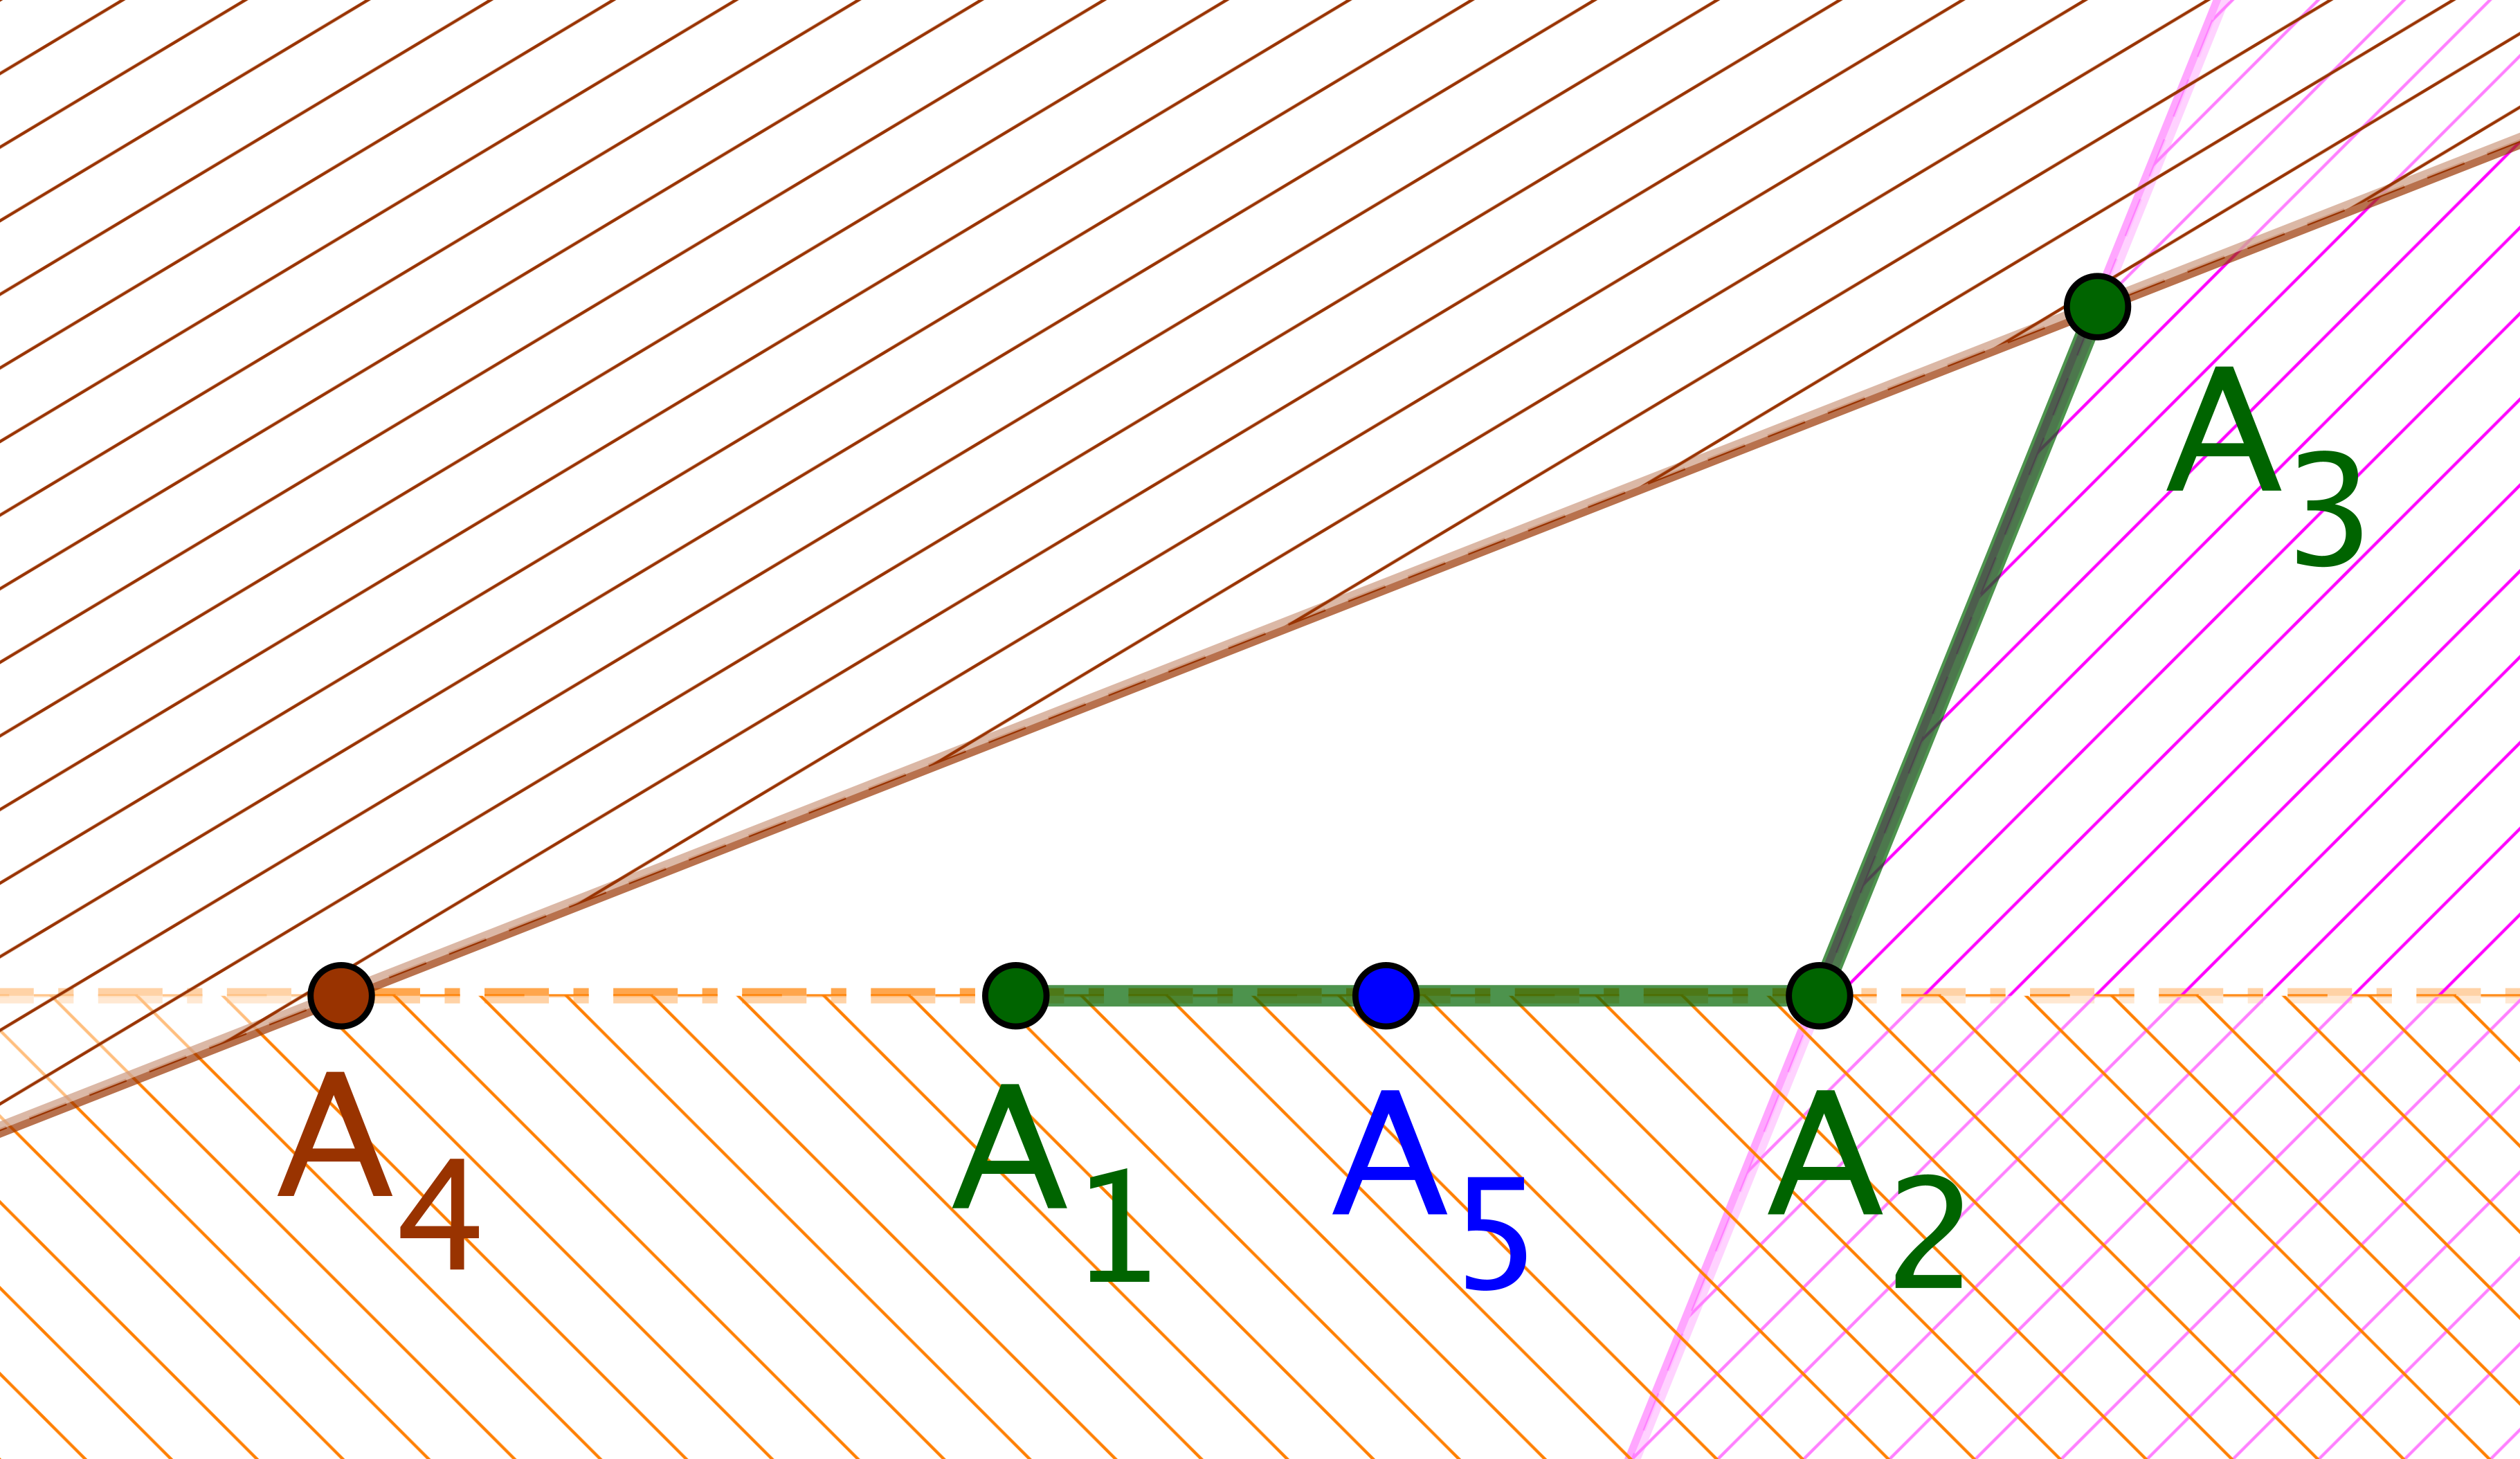
\includegraphics[scale=.4]{content/polygon/at-least-one/conv-det-A5-1.png}
        	    
        	\smallskip
            Cas 1-1.
            
            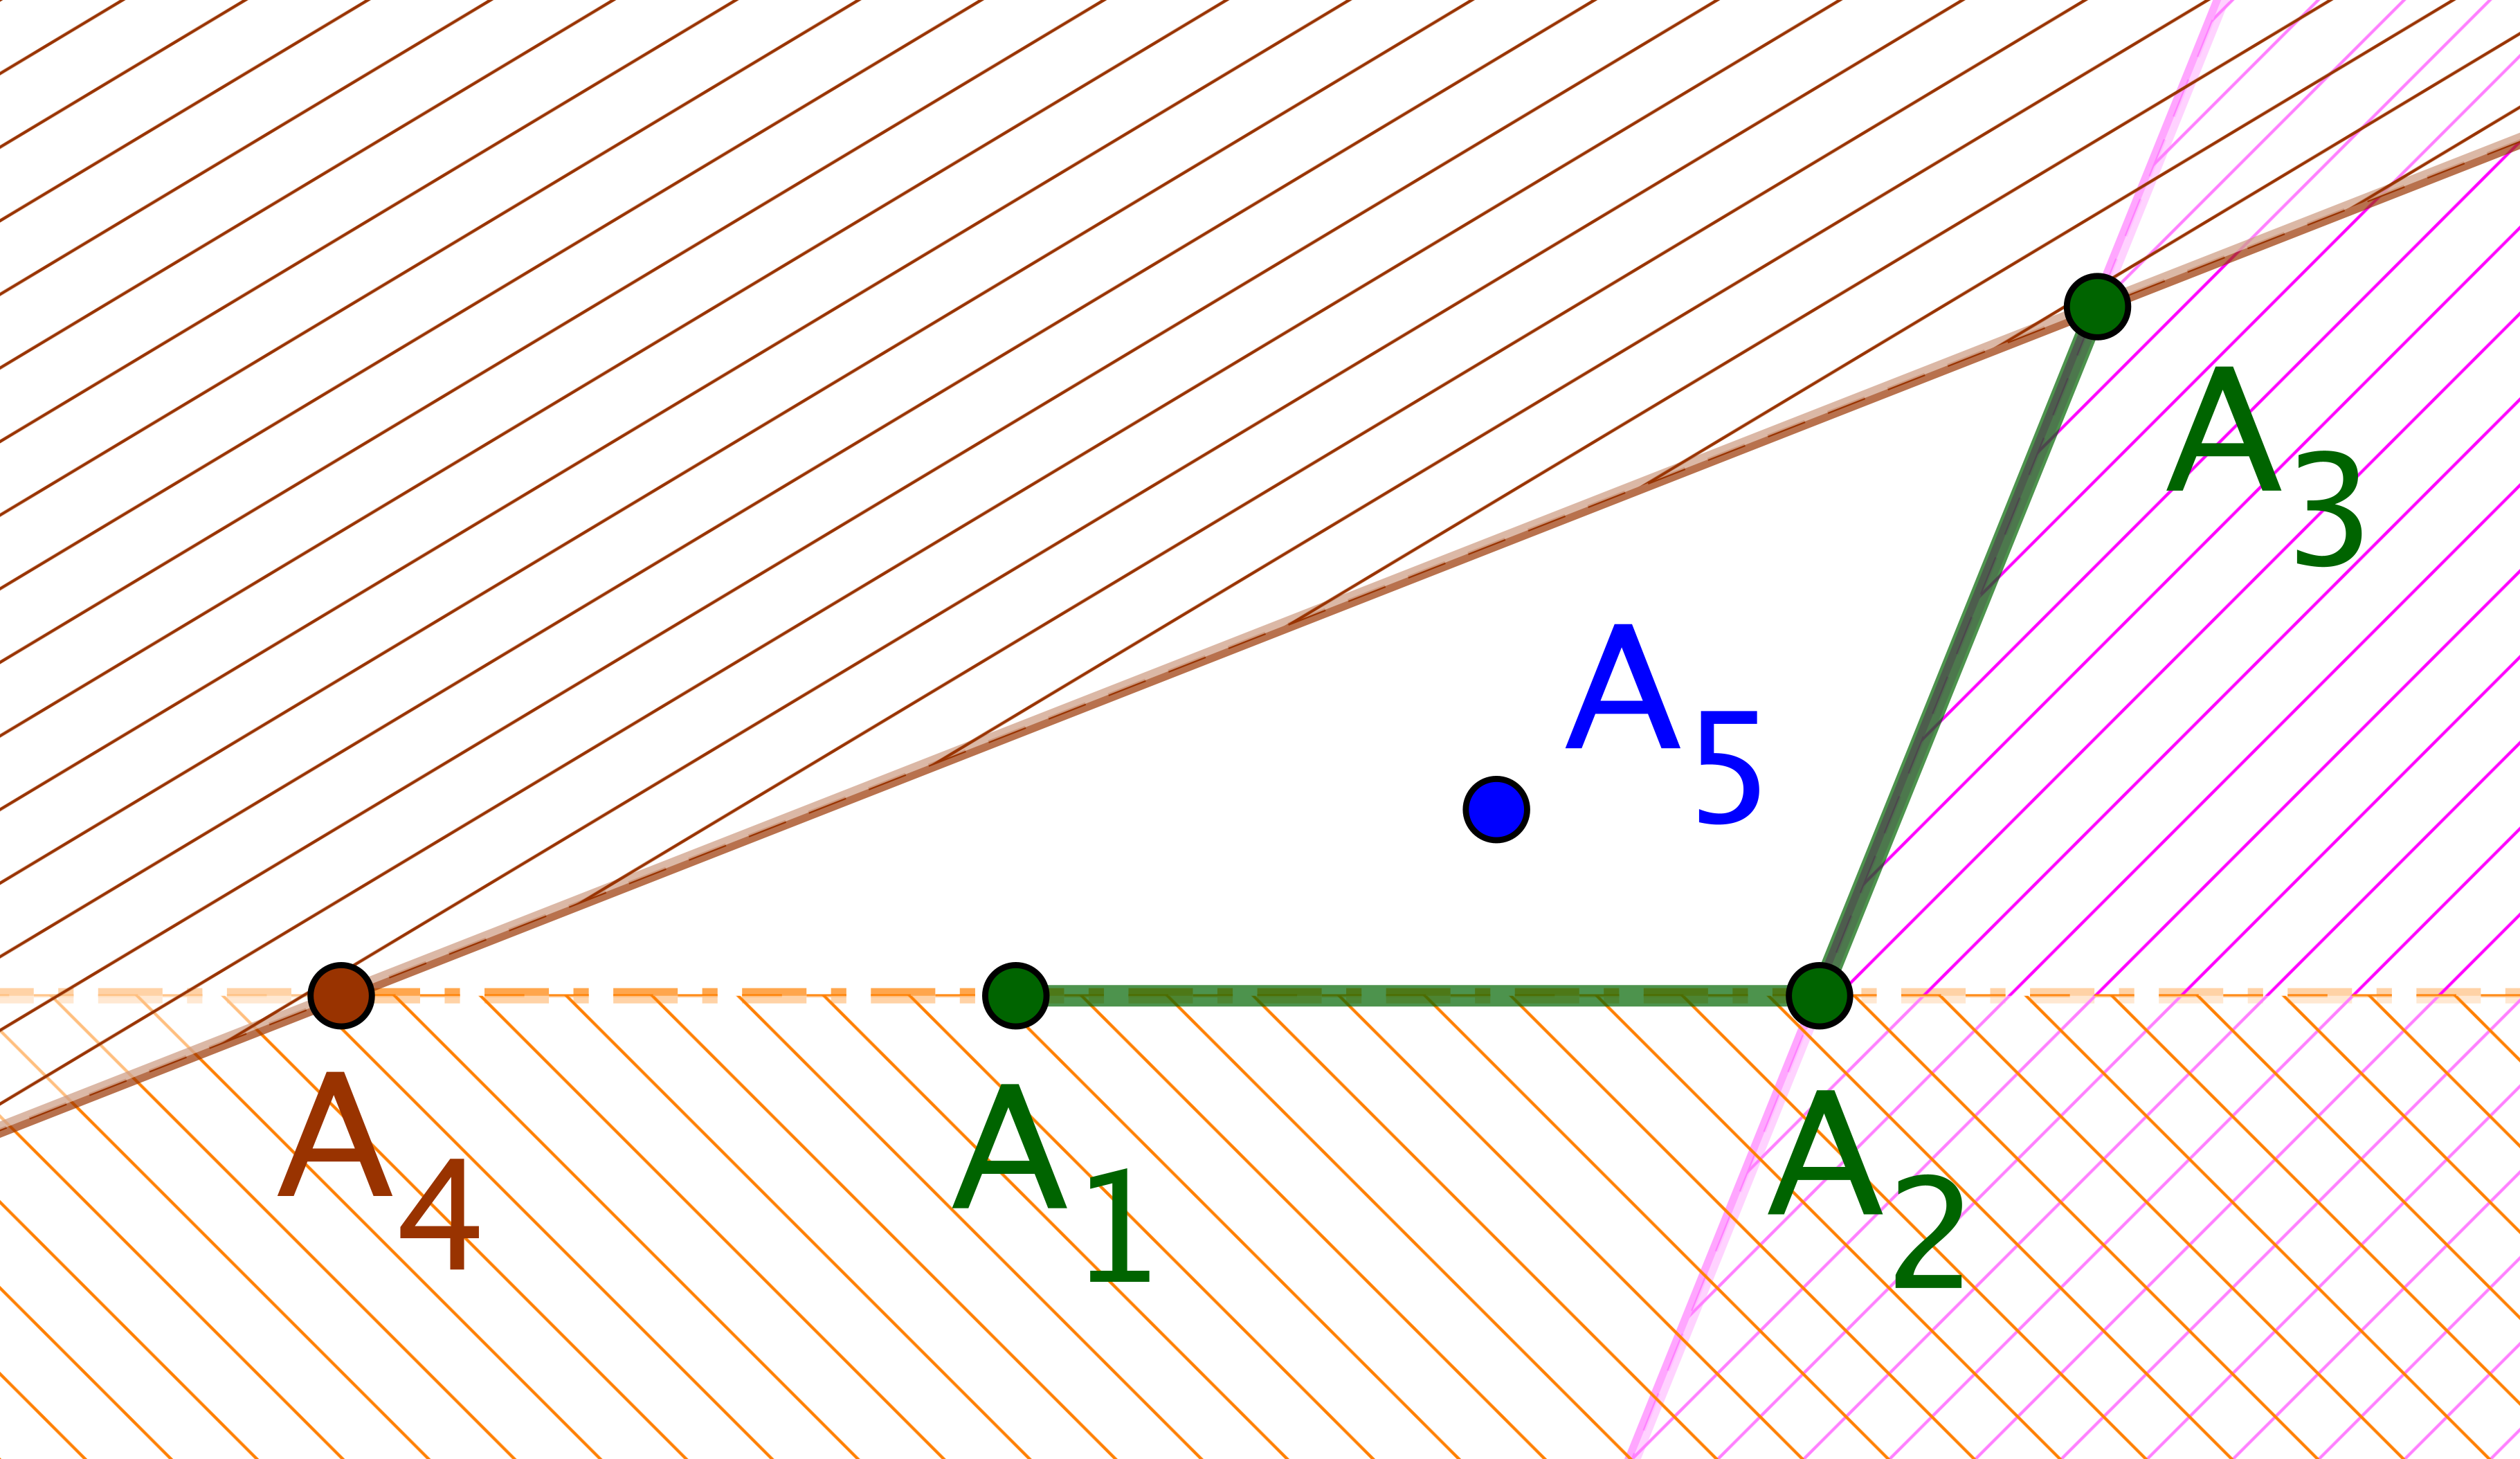
\includegraphics[scale=.4]{content/polygon/at-least-one/conv-det-A5-2.png}
        	    
        	\smallskip
            Cas 1-2.
        \end{multicols}
    
		\noindent
		Le cas 1-2 est impossible par raison de convexité, car $(A_4 A_5)$ sépare les points $A_3$ et $A_2$.
		Notons que dans le cas 1-1, il est possible d'avoir $A_5 \in {]A_4 A_1[}$.
		Comme $A_5 \in (A_1 A_2)$, nous devons avoir $n \geq 6$, 
		mais $A_6$ ne peut être ni à l'intérieur du triangle $A_2 A_3 A_4$ par convexité,
		ni sur la droite $(A_1 A_2)$, car $A_4$, $A_5$ et $A_6$ ne peuvent pas être alignés.
		Cette situation contradictoire montre que
		$\det \big( \vect{\primeit{A}_1 \primeit{A}_2}, \vect{\primeit{A}_1 \primeit{A}_4} \big) > 0$.
		En continuant de même, de proche en proche, nous arrivons à
		$\det \big( \vect{\primeit{A}_1 \primeit{A}_2}, \vect{\primeit{A}_1 \primeit{A}_k} \big) > 0$
		pour $k \in \ZintervalC{3}{n}$.


		\item En généralisant le raisonnement précédent,%
		\footnote{
		    Se souvenir de la définition \focus{cyclique} de la suite $(\primeit{A}_i)$.
		}
		nous avons
		$\det \big( \vect{\primeit{A}_i \primeit{A}_{i+1}}, \vect{\primeit{A}_i \primeit{A}_k} \big) > 0$
		pour tout couple $(i, k) \in \ZintervalC{1}{n}^2$ vérifiant $k \notin \setgene{i ; i+1}$.
	\end{itemize}

    \medskip
    
    \noindent
    Le cas négatif se traite de façon similaire.
\end{proof}


% ----------------------- %


Nous allons établir une réciproque élargie du résultat précédent. Ce nouveau fait, le plus technique à justifier, va nous rendre un grand service par la suite.%
\footnote{
    Pourquoi s'attarder sur des inégalités larges? Parce que nous allons travailler dans un ensemble compact, et donc fermé, de \ncycles.
    Pour garder des \ngones, nous devrions utiliser des non-égalités, mais ceci nous ferait sortir du cadre fermé qui nous intéresse.
    Nous n'avons pas le choix!
}


\begin{fact} \label{conv-from-non-neg-det}
    Soit $\setproba{L} = A_1 A_2 \cdots A_n$ un \ncycle\ vérifiant l'une des alternatives suivantes.
    %
	\begin{itemize}
		\item $\forall (i, k) \in \ZintervalC{1}{n}^2$,
		$\det \big( \vect{\primeit{A}_i \primeit{A}_{i+1}}, \vect{\primeit{A}_i \primeit{A}_k} \big) \geq 0$.

		\item $\forall (i, k) \in \ZintervalC{1}{n}^2$,
		$\det \big( \vect{\primeit{A}_i \primeit{A}_{i+1}}, \vect{\primeit{A}_i \primeit{A}_k} \big) \leq 0$.
    \end{itemize}
    
    Sous l'une de ces hypothèses, l'une des assertions ci-après est validée.
    %
	\begin{enumerate}[label=\roman*.]
		\item $\setproba{L}$ est totalement dégénéré.

		\item Il existe un \kgone\ convexe $\setproba{C}$ tel que
		$k \leq n$, 
		$\cyclelen{\setproba{C}} \leq \cyclelen{\setproba{L}}$
		et
		$\sarea{\setproba{C}} = \sarea{\setproba{L}}$.
		$\setproba{C}$ se construit en retirant, si nécessaire, des sommets de $\setproba{L}$, sans modifier l'ordre de parcours pour les sommets gardés.
		De plus,
		si $\primeit{A}_i$ et $\primeit{A}_k$ sont deux sommets consécutifs de $\setproba{C}$,
		alors les sommets $\primeit{A}_j$, pour $j \in \ZintervalC{i}{k}$, sont les seuls situés sur $[\primeit{A}_i \primeit{A}_k]$.
    \end{enumerate}
\end{fact}


\begin{proof}
    Par symétrie des alternatives, nous pouvons nous concentrer sur le cas positif,%
    \footnote{
        On pourrait aussi invoquer des cycles opposés.
    }
    c'est-à-dire supposer que 
    $\forall (i, k) \in \ZintervalC{1}{n}^2$,
	$\det \big( \vect{\primeit{A}_i \primeit{A}_{i+1}}, \vect{\primeit{A}_i \primeit{A}_k} \big) \geq 0$.
	%
	Seul le cas $\setproba{L}$ non totalement dégénéré requiert notre attention.
	%
	L'idée de la construction est simple: il s'agit de chercher des sommets extrémaux, c'est-à-dire qui \focus{forment un angle}. Nous allons raisonner algorithmiquement en utilisant
	une variable $i$ initialisée à $1$, 
	et
	une liste $\onelist{C}$, initialement vide, pour stocker les sommets \og utiles \fg\ à la fabrication du \kgone\ convexe final.
	%
	\begin{enumerate}[label=\fbox{\small\bfseries\textsf{A\kern.25pt\arabic*}}]
    	\item \label{algo-kgone-start}
	    Si 
		$\det \big( \vect{\primeit{A}_i \primeit{A}_{i+1}}, \vect{\primeit{A}_i \primeit{A}_{i+2}} \big) > 0$,
		nous ajoutons $\primeit{A}_{i+1}$ à la fin de la liste $\onelist{C}$,
		puis nous passons directement à l'action \ref{algo-kgone-loop-back}\,.


    	\item \label{algo-kgone-remove-vertices}
        Sinon, il existe 
	    $m \in \NN_{>i+2}$ minimal tel que
		$\det \big( \vect{\primeit{A}_i \primeit{A}_{i+1}}, \vect{\primeit{A}_i \primeit{A}_m} \big) > 0$, car $\setproba{L}$ n'est pas totalement dégénéré.
        %
        \begin{center}
        	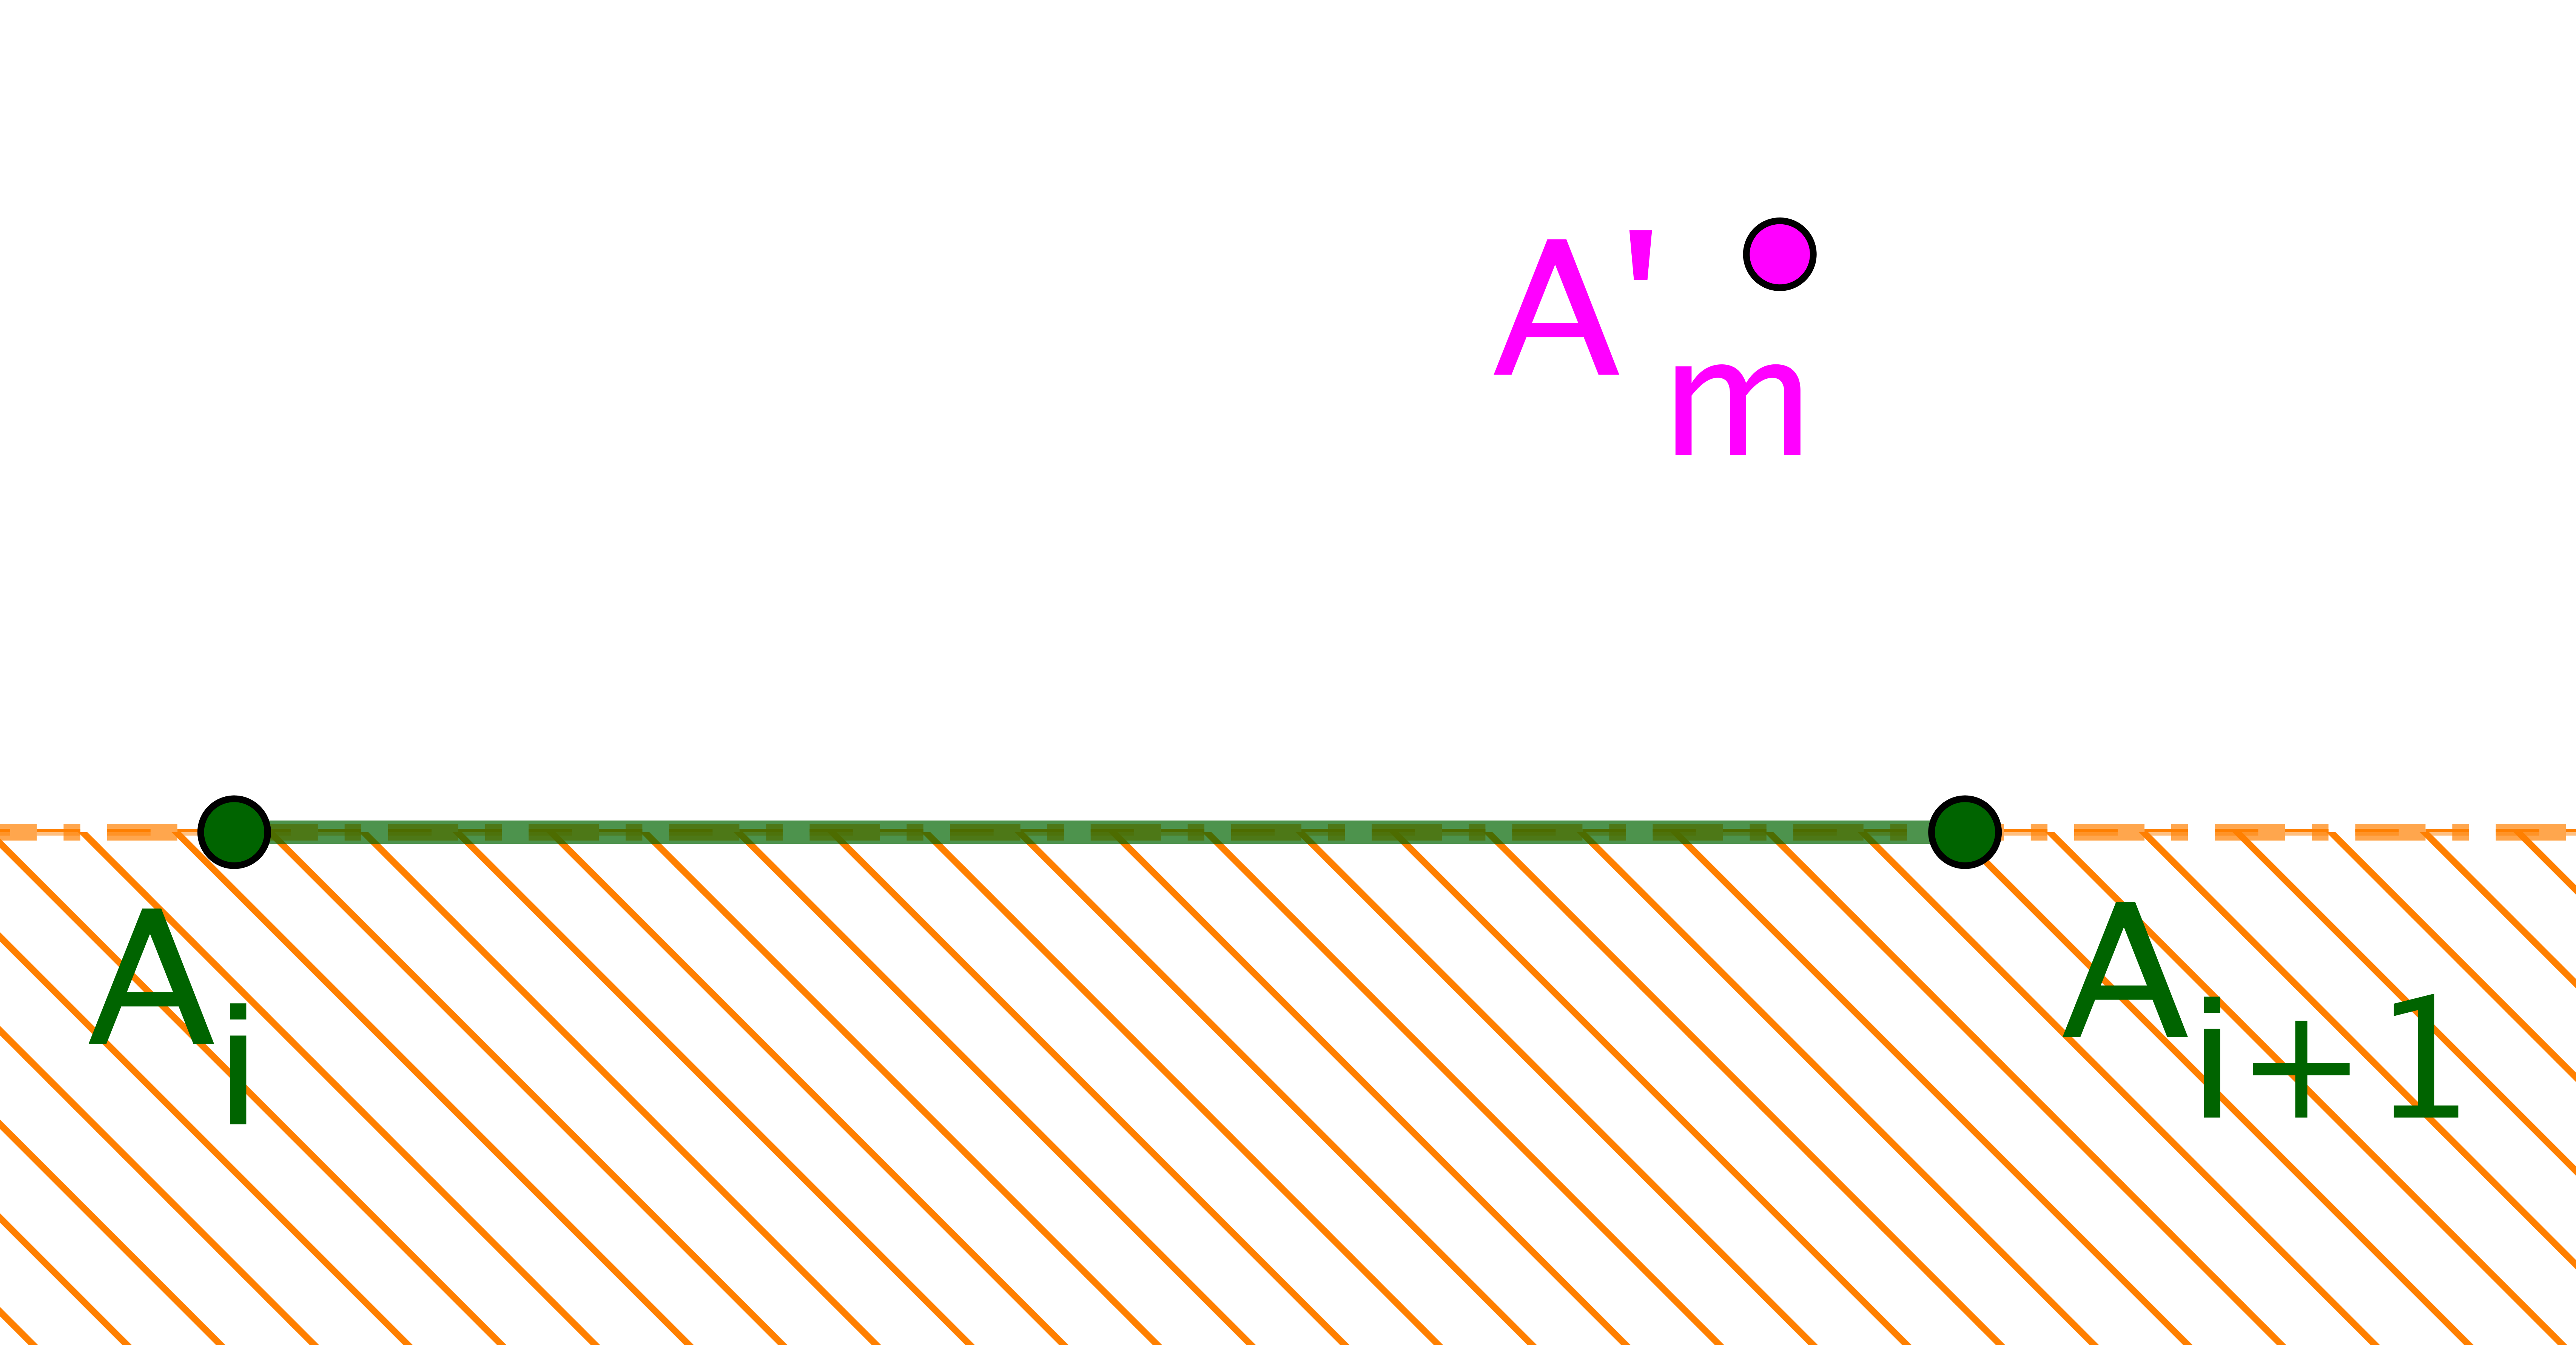
\includegraphics[scale=.4]{content/polygon/at-least-one/algo-kgone-remove-vertices.png}
        \end{center}
        
        \noindent
        Nous arrivons aux constatations suivantes.
        %
        \begin{itemize}
            \item Les points $\primeit{A}_i$, $\primeit{A}_{m-1}$ et $\primeit{A}_m$ ne sont pas alignés, et par conséquent deux à deux distincts.
            
            \item Comme 
            $\forall j \in \ZintervalC{1}{n}$,
            $\det \big( \vect{\primeit{A}_{m-1} \primeit{A}_m}, \vect{\primeit{A}_{m-1} \primeit{A}_{j}} \big) \geq 0$, 
            nous avons
            $\primeit{A}_{j} \in ( \primeit{A}_i , \primeit{A}_{m-1} ]$,
            pour $j \in \ZintervalO{i}{m-1}$.%
            \footnote{
        	    Le point $\primeit{A}_{m-1}$ est le plus à droite sur notre schéma.
            }

            \item L'évaluation de l'aire algébrique via le point de calcul $\primeit{A}_{m-1}$ peut se passer des sommets $\primeit{A}_j$ pour $j \in \ZintervalO{i}{m-1}$, par raison d'alignement.

            \item Ignorer des sommets, tout en conservant l'ordre de parcours, pour former un nouveau cycle $\setproba{L}^{\,\prime}$, donne $\cyclelen{\setproba{L}^{\,\prime}} \leq \cyclelen{\setproba{L}} $.
        \end{itemize}
        
        \noindent
        Les constatations précédentes justifient l'ajout de
        $\primeit{A}_{m-1}$ à la fin de la liste $\onelist{C}$, uniquement si $\primeit{A}_{m-1}$ n'est pas dans cette liste,%
        \footnote{
        	La justification de l'algorithme, donnée un peu plus bas, montrera la possibilité d'avoir un doublon dans la liste $\onelist{C}$.
        }
        puis de poser $i = m - 2$, puisque nous augmentons $i$ de $1$ juste après.

	
		\item \label{algo-kgone-loop-back}
		Ajoutons $1$ à $i$.
		Si $i \geq n+1$, nous avons fini, sinon nous retournons à l'action \ref{algo-kgone-start}\,.
    \end{enumerate}
    

    \medskip

    
    Commençons par justifier que l'algorithme s'arrête sans entrer dans une boucle infinie.
    Tant que l'indice $m$ de l'étape \ref{algo-kgone-remove-vertices} vérifie $m \leq n$, il n'y a aucune difficulté, car $i$ augmente, et les sommets ajoutés se placent \focus{avant} l'origine $A_1$ du \ncycle\ initial $\setproba{L}$ sans empiéter sur les \focus{premiers} sommets. Supposons avoir $m \in \ZintervalO{n}{n+i}$ pour un indice $i$, où forcément $i > 1$, et par conséquent $\primeit{A}_i$ a été stocké dans la liste $\onelist{C}$.
    %
    \begin{itemize}
        \item Commençons par noter l'existence de $A_1$, $A_r$ et $A_s$ non alignés avec $A_r$ et $A_s$ stockés dans $\onelist{C}$.
        En effet,
        $A_r$ vient de l'application de l'algorithme à $i = 1$, 
        puis
        $A_s$ s'obtient avec $i = r$.


        \item Supposons que $i = s$. 
        Pour $j \in \ZintervalC{s+1}{n}$, les points $\primeit{A}_j$ sont sur la droite $( \primeit{A}_s \primeit{A}_1)$, 
        et ensuite plus généralement pour $j \in \ZintervalO{s}{m}$. 
        Le schéma suivant montre sans ambigüité qu'alors
        $\primeit{A}_{m-1} = \primeit{A}_1$.%
        \footnote{
            $\primeit{A}_{m-1} \neq \primeit{A}_1$ contredirait la condition de positivité large sur les déterminants.
        }
        Dès lors, $m = n+2$, d'où l'ajout de $\primeit{A}_1$ à la fin de la liste $\onelist{C}$, puis l'arrêt de l'algorithme à l'étape suivante.
        %
        \begin{center}
        	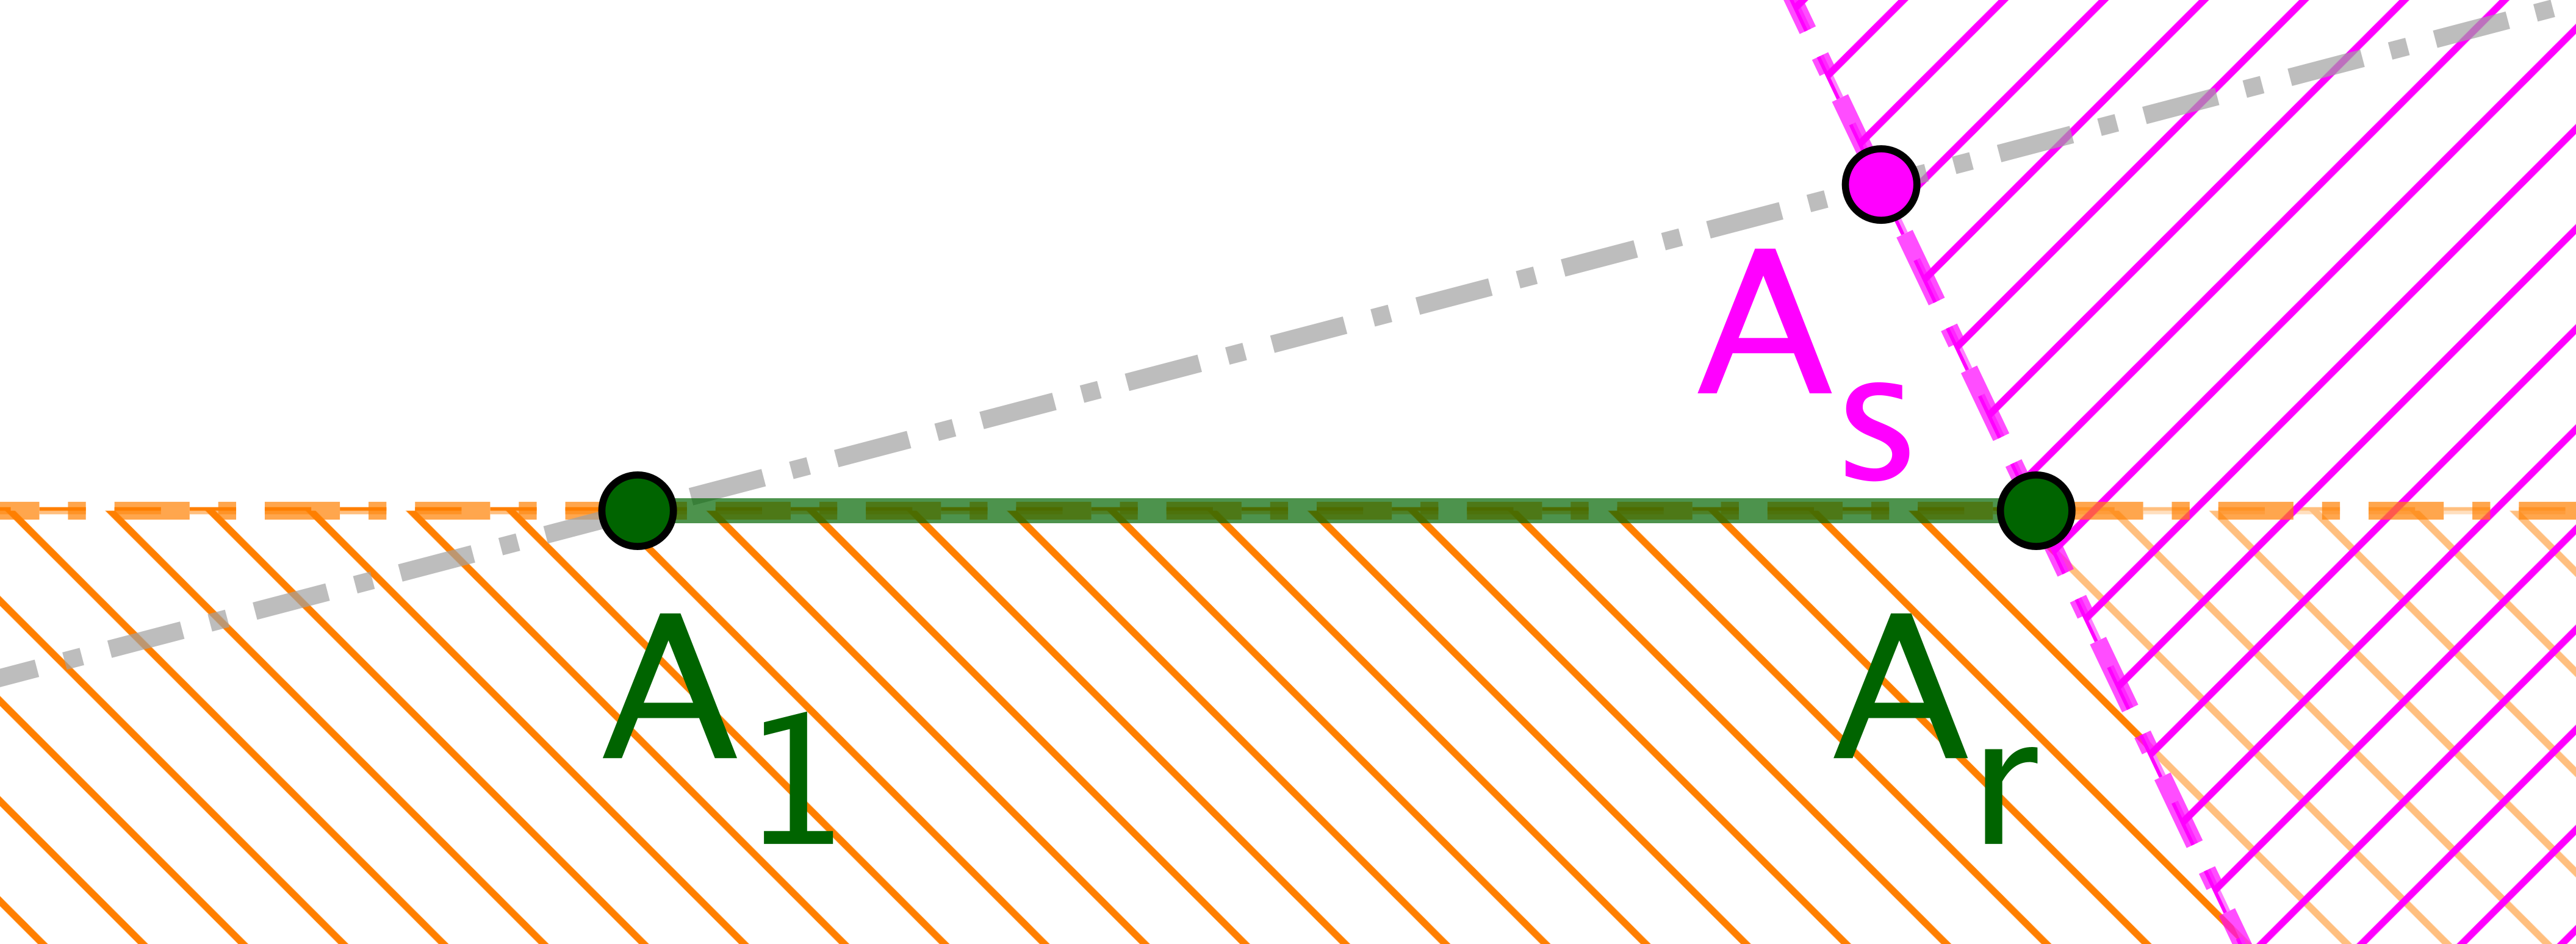
\includegraphics[scale=.4]{content/polygon/at-least-one/algo-kgone-terminate-1.png}
        \end{center}


        \item Le raisonnement précédent fonctionne plus généralement lorsque $\primeit{A}_i \notin (\primeit{A}_1 \primeit{A}_r)$.


        \item Il reste le cas où $\primeit{A}_i \in (\primeit{A}_1 \primeit{A}_r)$.
       Ceci nous donne le schéma suivant, où
       $\primeit{A}_i \in [\primeit{A}_1 \primeit{A}_r]$ est possible, a priori. 
        %
        \begin{center}
        	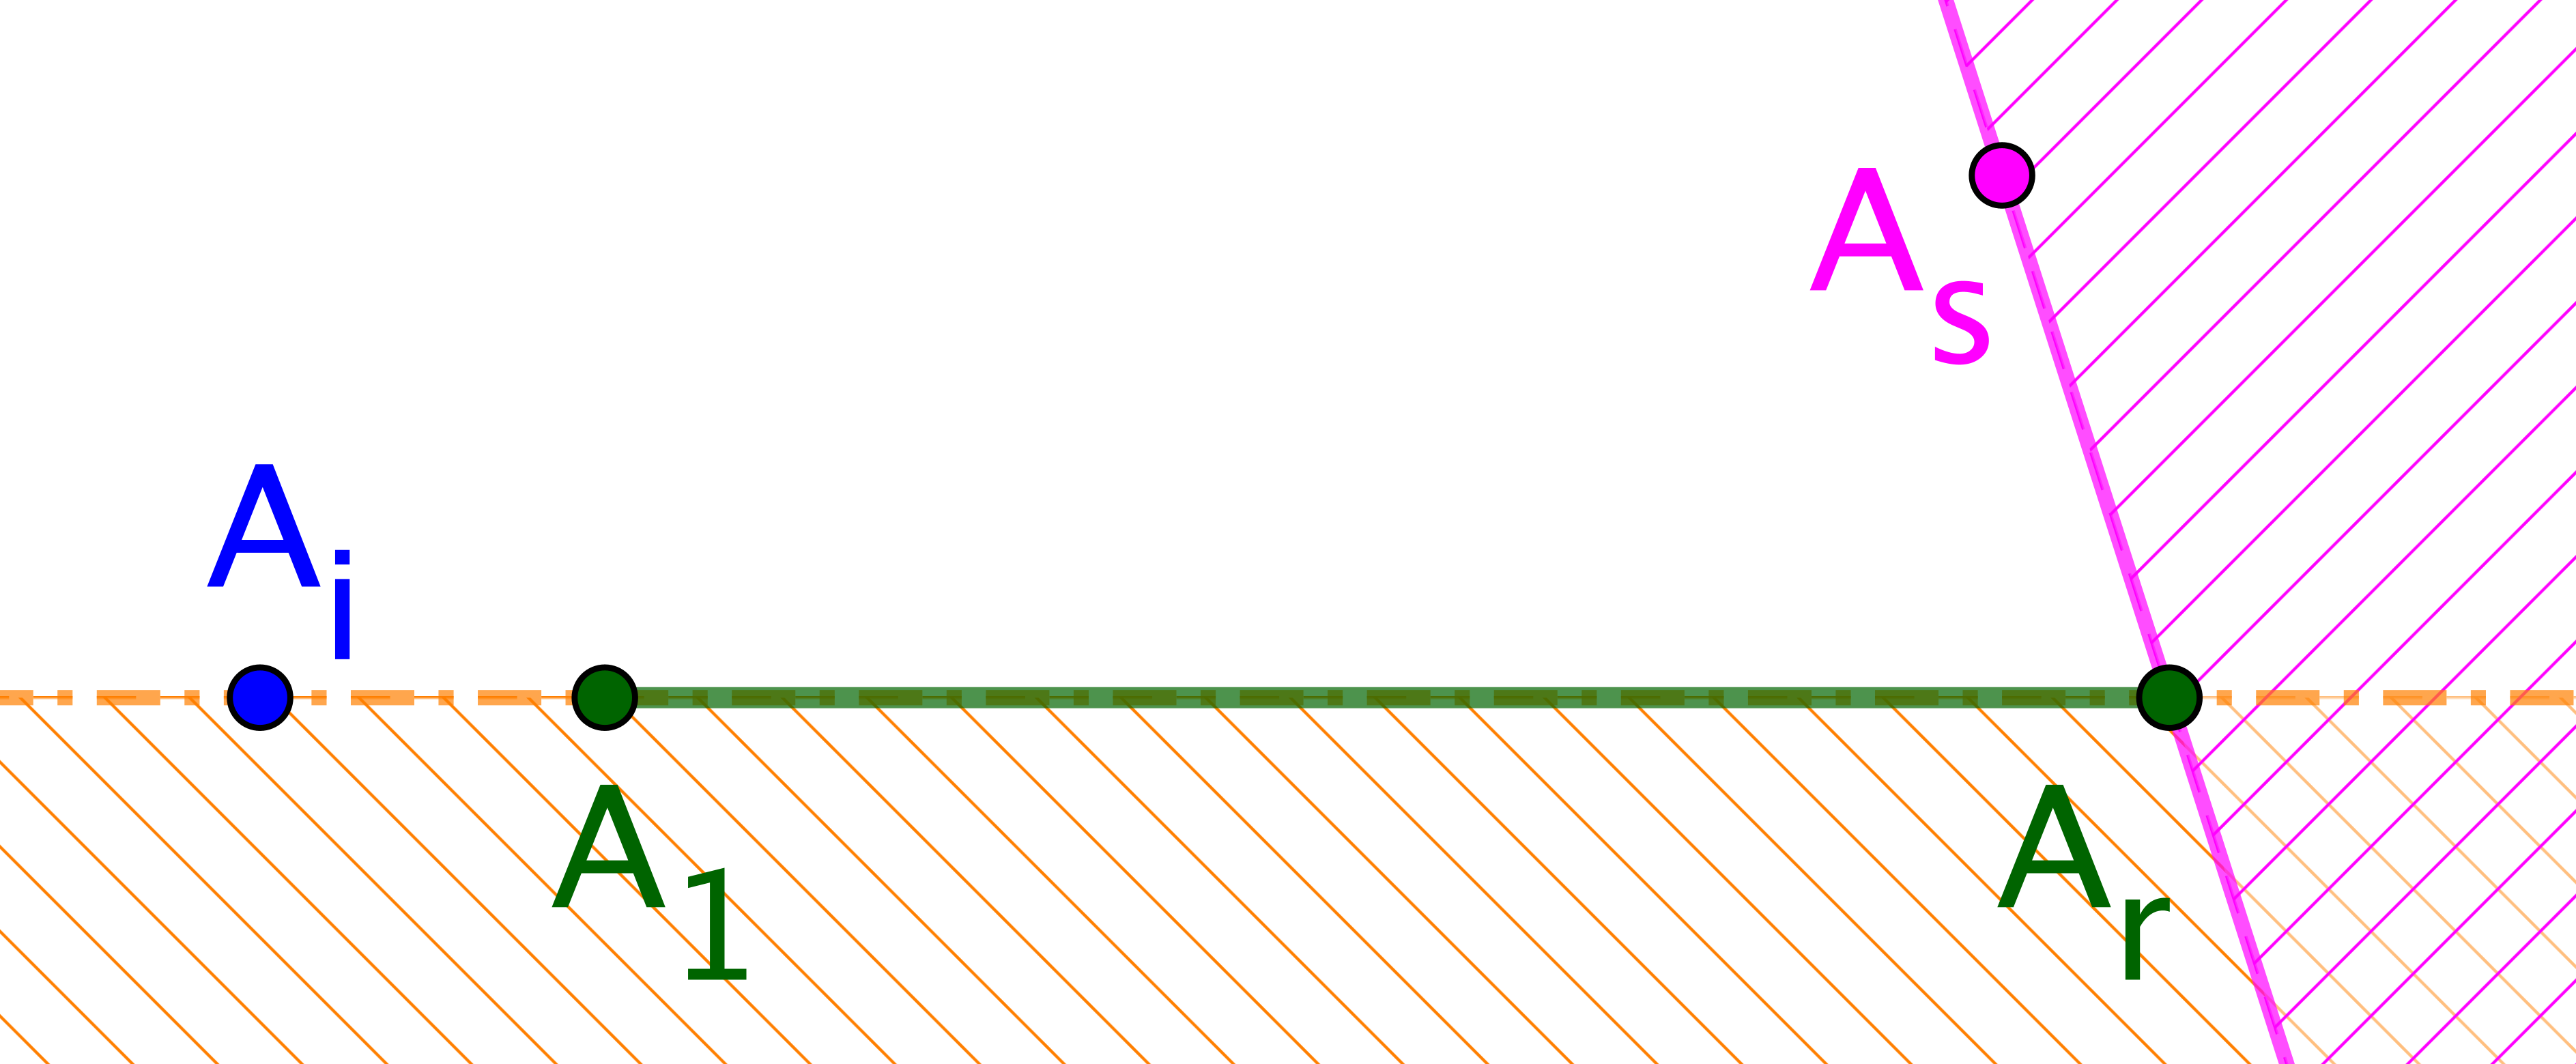
\includegraphics[scale=.4]{content/polygon/at-least-one/algo-kgone-terminate-2.png}
        \end{center}
        
        \noindent
        L'algorithme assure l'existence d'un point $\primeit{A}_p \notin ( \primeit{A}_1 , \primeit{A}_r )$ stocké dans $\onelist{C}$ et \focus{précédent} $\primeit{A}_i$,
        tel que tout point entre $\primeit{A}_p$ et $\primeit{A}_i$ soit sur $(\primeit{A}_p \primeit{A}_i)$.
        Nous arrivons au schéma plus précis ci-dessous, où
        $\primeit{A}_1 \in [ \primeit{A}_i , \primeit{A}_r ]$
        par positivité large des déterminants
        $\det \big( \vect{\primeit{A}_p \primeit{A}_{p+1}}, \vect{\primeit{A}_p \primeit{A}_k} \big)$,
        avec la possibilité d'avoir $\primeit{A}_p = \primeit{A}_s$.
        %
        \begin{center}
        	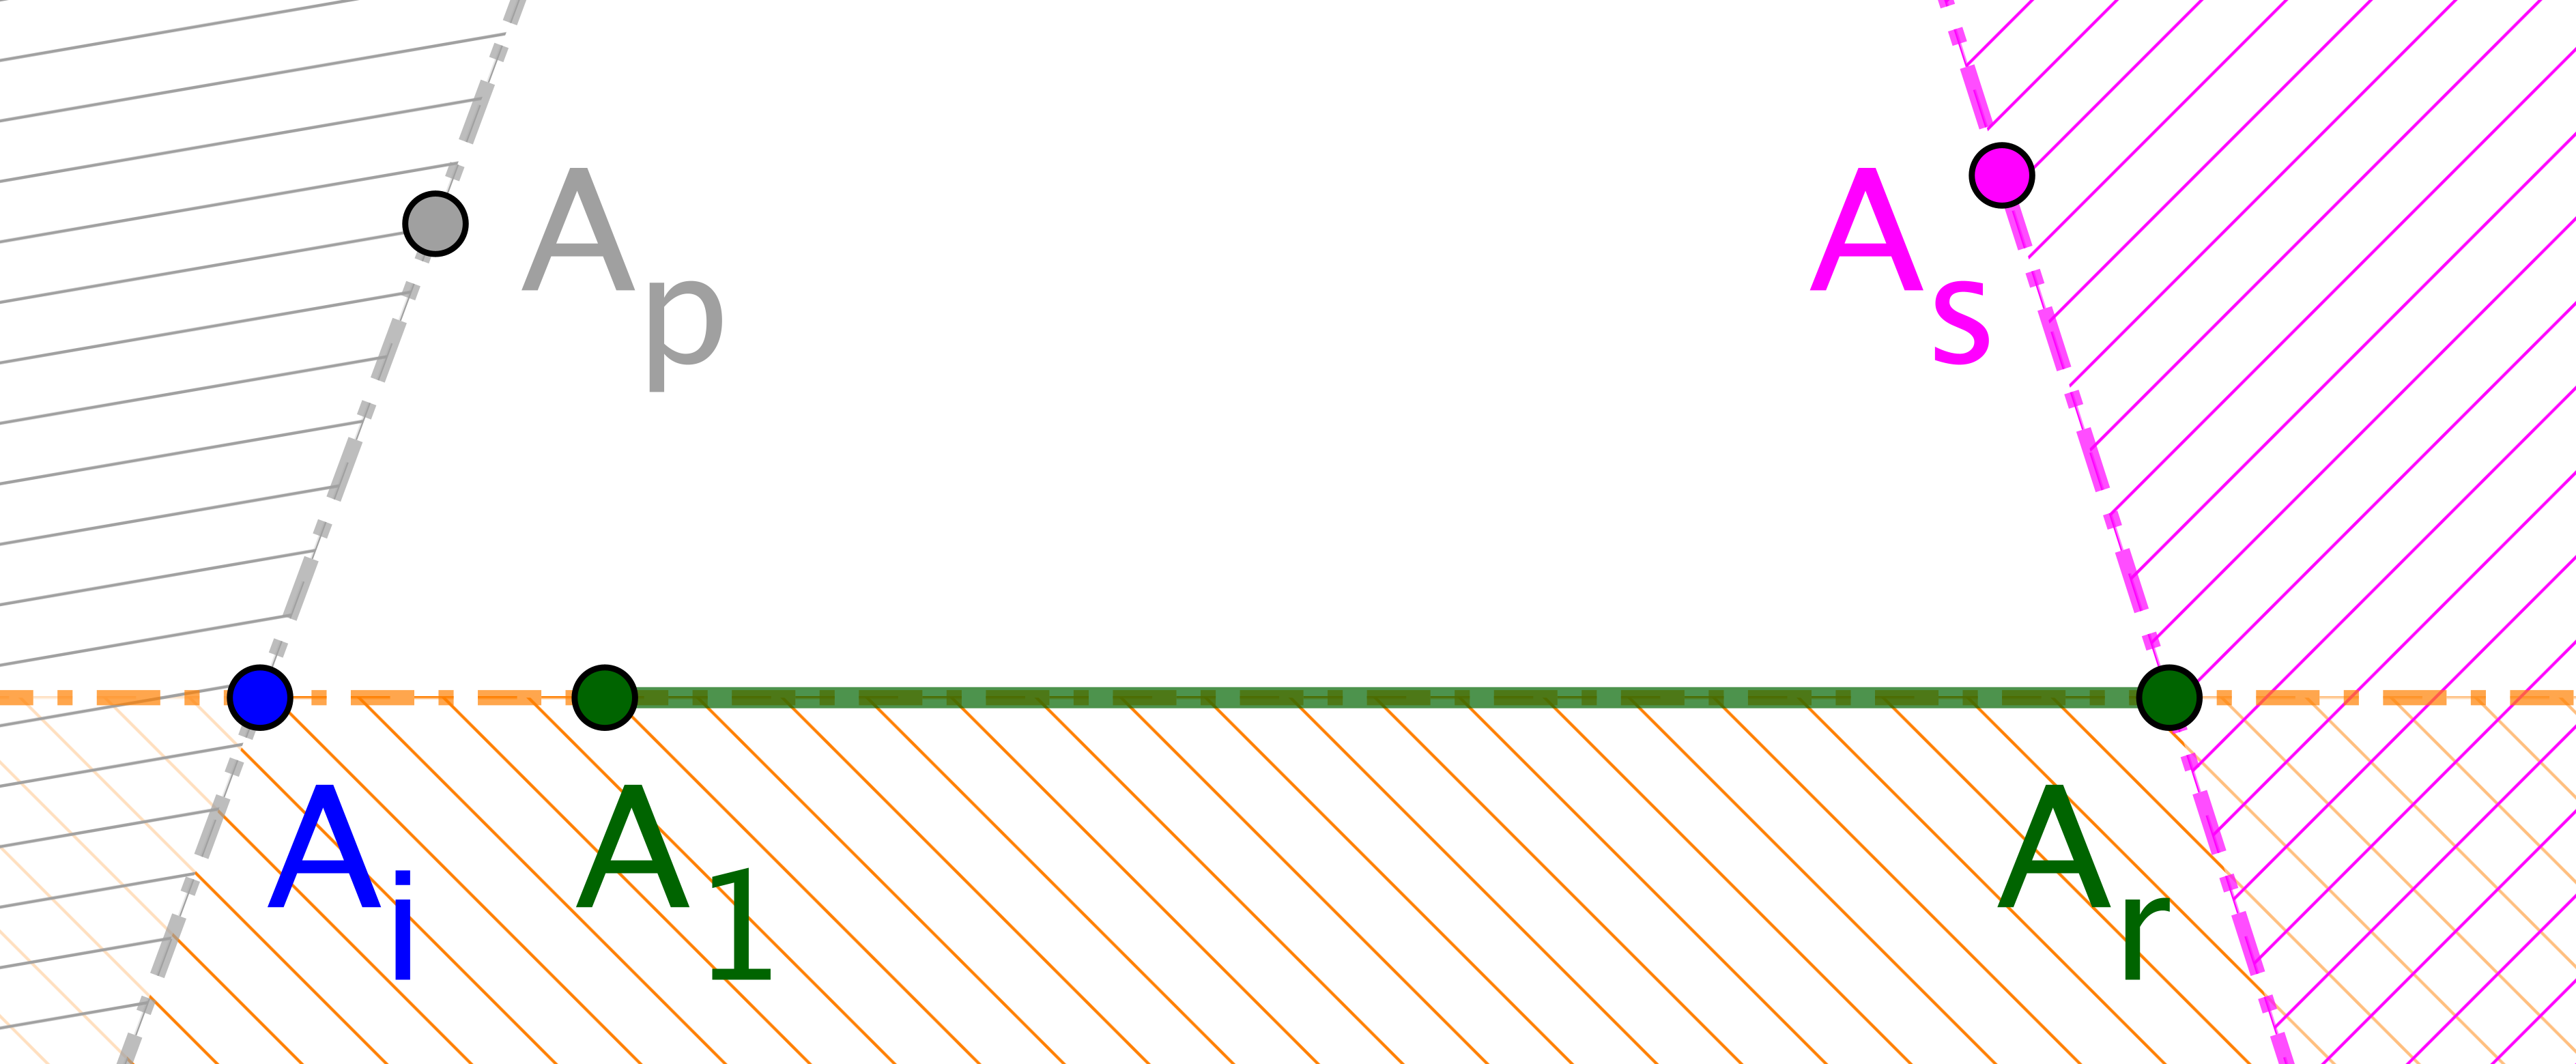
\includegraphics[scale=.4]{content/polygon/at-least-one/algo-kgone-terminate-3.png}
        \end{center}
        
        \noindent
        Ici,
        $\primeit{A}_r$ est déjà présent dans $\onelist{C}$,
        donc l'algorithme s'arrêtera après avoir juste modifié $i$ en $(n + r)$.
        Notons que les points de $\primeit{A}_{i+1}$ à $\primeit{A}_{r-1}$ sont \focus{mangés} comme attendu.
    \end{itemize}
    
    
    \medskip
    
    
    Il faut aussi justifier que la liste $\onelist{C}$, lue de gauche à droite, donnera les sommets du \kgone\ convexe $\setproba{C}$ cherché.
    %
    \begin{itemize}
        \item Par construction, deux sommets \focus{consécutifs} $\primeit{A}_r$ et $\primeit{A}_s$ de $\setproba{C}$, sont tels que tout point du cycle initial $\setproba{L}$ situé entre $\primeit{A}_r$ et $\primeit{A}_s$ se trouve sur le segment $[\primeit{A}_r \primeit{A}_s]$.
        En ignorant ces points, on fait donc diminuer, au sens large, la longueur du \ncycle, mais sans modifier la valeur de l'aire algébrique, cette dernière étant calculable depuis $\primeit{A}_r$, ou $\primeit{A}_s$.
        Donc
        $\cyclelen{\setproba{C}} \leq \cyclelen{\setproba{L}}$
		et
		$\sarea{\setproba{C}} = \sarea{\setproba{L}}$


        \item Par construction, trois sommets \focus{consécutifs} $\primeit{A}_q$, $\primeit{A}_r$ et $\primeit{A}_s$ de $\setproba{C}$, sont tels que $\det \big( \vect{\primeit{A}_q \primeit{A}_{r}}, \vect{\primeit{A}_q \primeit{A}_s} \big) > 0$. 
        En particulier, ces trois sommets \focus{consécutifs} ne sont pas alignés.
        Dès lors, $\setproba{C}$ est un \kgone, et il est aussi convexe. 
    \end{itemize}

	
	Enfin, la preuve de l'algorithme a montré que pour $\primeit{A}_i$ et $\primeit{A}_k$ deux sommets consécutifs de $\setproba{C}$, les sommets $\primeit{A}_j$, pour $j \in \ZintervalC{i}{k}$, sont les seuls situés sur $[\primeit{A}_i \primeit{A}_k]$.
\end{proof}


% ----------------------- %


%\newpage
%

Le résultat qui suit est juste là pour simplifier la justification du fait \ref{at-least-one-ngone-convex} à venir qui est la raison d'être de cette section.


\begin{fact} \label{at-least-one-ncycle}
    Soient $n \in \NN_{\geq3}$,
    $\ell \in \RRsp$,
    $\pvaxes{O | i | j}$ un repère orthonormé direct du plan
    et
    $\setproba{U} \subset \RR^{2n}$ l'ensemble des uplets de coordonnées $\big( x(A_1) ; y(A_1) ; \dots ; x(A_n) ; y(A_n) \big)$ où $\setproba{L} = A_1 A_2 \cdots A_n$ désigne un \ncycle\ vérifiant les conditions suivantes.
    %
    \begin{itemize}
        \item $\cyclelen{\setproba{L}} = \ell$.
    
        \item $\forall (i, k) \in \ZintervalC{1}{n}^2$,
		$\det \big( \vect{\primeit{A}_i \primeit{A}_{i+1}}, \vect{\primeit{A}_i \primeit{A}_k} \big) \geq 0$.
    \end{itemize}
    
    Dès lors, la fonction $\alpha: \setproba{U} \rightarrow \RR$, qui à un uplet de $\setproba{U}$ associe l'aire algébrique du \ncycle\ qu'il représente, est une fonction admettant au moins un maximum, qui est positif strict.
\end{fact}


\begin{proof}
     $\setproba{U}$ est fermé dans $\RR^{2n}$, car les conditions le définissant le sont, et il est borné, car inclus dans la boule fermée de centre $\pt{O}$ et de rayon $\ell$,
     donc $\setproba{U}$ est un compact de $\RR^{2n}$.
     De plus, $\alpha$ est continue d'après le fait \ref{sarea-cont}.
     Donc, par continuité et compacité, $\alpha$ admet un maximum sur $\setproba{U}$, celui-ci étant positif strict pour les raisons suivantes où $\setproba{R}$ désigne un \nreg\ convexe.
    %
    \begin{itemize}
        \item Il est connu, et facile de démontrer, que pour tout \nreg\ convexe $\setproba{R}$, nous avons 
        $\perim{\setproba{R}} = 2 n \sin (\frac{\pi}{n}) \rho$
		et
		$\area{\setproba{R}} = n \sin (\frac{\pi}{n})  \cos (\frac{\pi}{n}) \rho^2$
		où $\rho$ désigne le rayon du cercle circonscrit à $\setproba{R}$.
		Ceci donne un \nreg\ convexe $\setproba{R}$ de longueur $\ell$, et d'aire non nulle.

		\item Via une translation, nous pouvons supposer $\setproba{R}$ d'origine $\pt{O}$.

        \item $\area{\setproba{R}} = \abs{\sarea{\setproba{R}}}$
		selon le fait \ref{sarea-ngone},
		et
		$\sarea{\setproba{R}^{\mathrm{op}}} = - \sarea{\setproba{R}}$ d'après le fait \ref{nline-rota-opp}.
		
		\item $\setproba{R} \in \setproba{U}$, ou $\setproba{R}^{\mathrm{op}} \in \setproba{U}$ selon le fait \ref{conv-pos-det}.
		
		\item Si $\setproba{R} \in \setproba{U}$, alors 
		$\setproba{R}$ est orienté positivement, 
		d'où $\sarea{\setproba{R}} \geq 0$, 
		et par conséquent $\sarea{\setproba{R}} = \area{\setproba{R}}$ 
		(c'est immédiat en utilisant le centre de gravité de $\setproba{R}$ comme point de calcul). 
		Nous avons une propriété similaire si $\setproba{R}^{\mathrm{op}} \in \setproba{U}$.
    \end{itemize}

	\null\vspace{-6ex}
\end{proof}


% ----------------------- %


Nous arrivons au résultat fondamental sur les \ngones\ convexes.


\begin{fact} \label{at-least-one-ngone-convex}
    Soit $n \in \NN_{\geq3}$ un naturel fixé.
    Parmi les \ngones\ convexes de longueur fixée, non nulle, il en existe au moins un d'aire maximale.
\end{fact}


\begin{proof}
    Notons $\ell > 0$ la longueur fixée,
    reprenons les notations du fait \ref{at-least-one-ncycle},
    et choisissons $\setproba{M} \in \setproba{U}$ maximisant l'aire algébrique sur $\setproba{U}$.
    Ce \ncycle\ ne peut être totalement dégénéré, car $\sarea{\setproba{M}} > 0$.
    Dès lors, pour tout \ngone\ convexe $\setproba{P}$ vérifiant $\cyclelen{\setproba{P}} = \ell$, nous pouvons raisonner comme suit. 
	%
	\begin{itemize}
		\item Comme pour le \nreg\ convexe $\setproba{R}$ de la preuve du fait \ref{at-least-one-ncycle},
		via une translation, nous pouvons supposer $\setproba{P}$ d'origine $\pt{O}$, puis nous avons
		soit $\setproba{P} \in \setproba{U}$ et $\sarea{\setproba{P}} = \area{\setproba{P}}$,
		soit $\cycleop{P} \in \setproba{U}$ et $\sarea{\cycleop{P}} = \area{\cycleop{P}}$.
		Comme, de plus, $\area{\cycleop{P}} = \area{\setproba{P}}$,
		nous pouvons supposer avoir $\setproba{P} \in \setproba{U}$,
		quitte à échanger $\setproba{P}$ et $\cycleop{P}$.


		\item Le fait \ref{conv-from-non-neg-det} donne un \kgone\ convexe $\setproba{C}$, où $k \leq n$, tel que
		$\cyclelen{\setproba{C}} \leq \cyclelen{\setproba{M}}$,
		ainsi que
		$\sarea{\setproba{C}} = \sarea{\setproba{M}}$.
		%
		Nous savons que pour deux sommets consécutifs $\primeit{A}_i$ et $\primeit{A}_k$ de $\setproba{C}$, seuls les sommets $\primeit{A}_j$, pour $j \in \ZintervalC{i}{k}$, sont situés sur $[\primeit{A}_i \primeit{A}_k]$.
		%
		Ceci nous amène aux deux alternatives suivantes donnant un \ngone\ convexe $\primeit{\setproba{C}}$ tel que 
		$\cyclelen{\primeit{\setproba{C}}} \leq \cyclelen{\setproba{M}}$
		et
		$\sarea{\primeit{\setproba{C}}} \geq \sarea{\setproba{M}} > 0$.
		%
		\begin{enumerate}
		    \item Si $M$ est déjà un \ngone\ convexe, alors $\setproba{C} = \setproba{M}$ et donc $\primeit{\setproba{C}} \eq[def] \setproba{C}$ convient.
		    

		    \item Sinon, forcément $\primeit{\setproba{C}}$ possède strictement moins de sommets que $\setproba{M}$, et par conséquent $\cyclelen{\setproba{C}} < \cyclelen{\setproba{M}}$.
		    Dans ce cas, 
		    le \ngone\ convexe $\primeit{\setproba{C}}$ vient du fait \ref{bigger-convex} ci-dessous appliqué 
		    au convexe $\setproba{C}$ 
		    avec 
		    $s = n - k$
		    et
		    $\delta = \cyclelen{\setproba{M}} - \cyclelen{\setproba{C}}$.
		\end{enumerate}


		\item Le choix de $\setproba{M}$ fait que 
		$\cyclelen{\primeit{\setproba{C}}} \leq \ell$
		et
		$\sarea{\primeit{\setproba{C}}} \geq \sarea{\setproba{P}}$.


		\item Selon le fait \ref{sarea-ngone},
		$\area{\primeit{\setproba{C}}} = \abs{\sarea{\primeit{\setproba{C}}}} = \sarea{\primeit{\setproba{C}}}$,
		donc l'inégalité
		$\sarea{\setproba{P}} \leq \sarea{\primeit{\setproba{C}}}$
		devient
		$\area{\setproba{P}} \leq \area{\primeit{\setproba{C}}}$.
		
		
		\item Pour conclure, notons que $\cyclelen{\primeit{\setproba{C}}} > 0$, donc une homothétie de rapport $\frac{\ell}{\cyclelen{\primeit{\setproba{C}}}} \geq 1$ fournit un \ngone\ convexe $\dbleprimeit{\setproba{C}}$ tel que
		$\cyclelen{\dbleprimeit{\setproba{C}}} = \ell$
		et
		$\area{\setproba{P}} \leq \area{\dbleprimeit{\setproba{C}}}$.
	\end{itemize}

	\null\vspace{-6ex}
\end{proof}


% ----------------------- %


Le fait suivant, utilisé dans la preuve précédente, nous sera aussi utile pour obtenir qu'un \ngone\ \focus{maximal} doit être convexe.


\begin{fact} \label{bigger-convex}
    XXXX
\end{fact}


\begin{proof}
    XXXX
    		    ceci conduisant à une situation comme la suivante où nous notons la possibilité d'ajouter autant de sommets manquant que nécessaire, la zone hachurée indiquant les points $M$ tels que 
		    $\det \big( \vect{\primeit{A}_i \primeit{A}_{i+1}}, \vect{\primeit{A}_i M} \big) < 0$, une zone ne contenant aucun sommet de $\setproba{M}$.
            %
            \begin{multicols}{2}
                \small\itshape\centering
           	    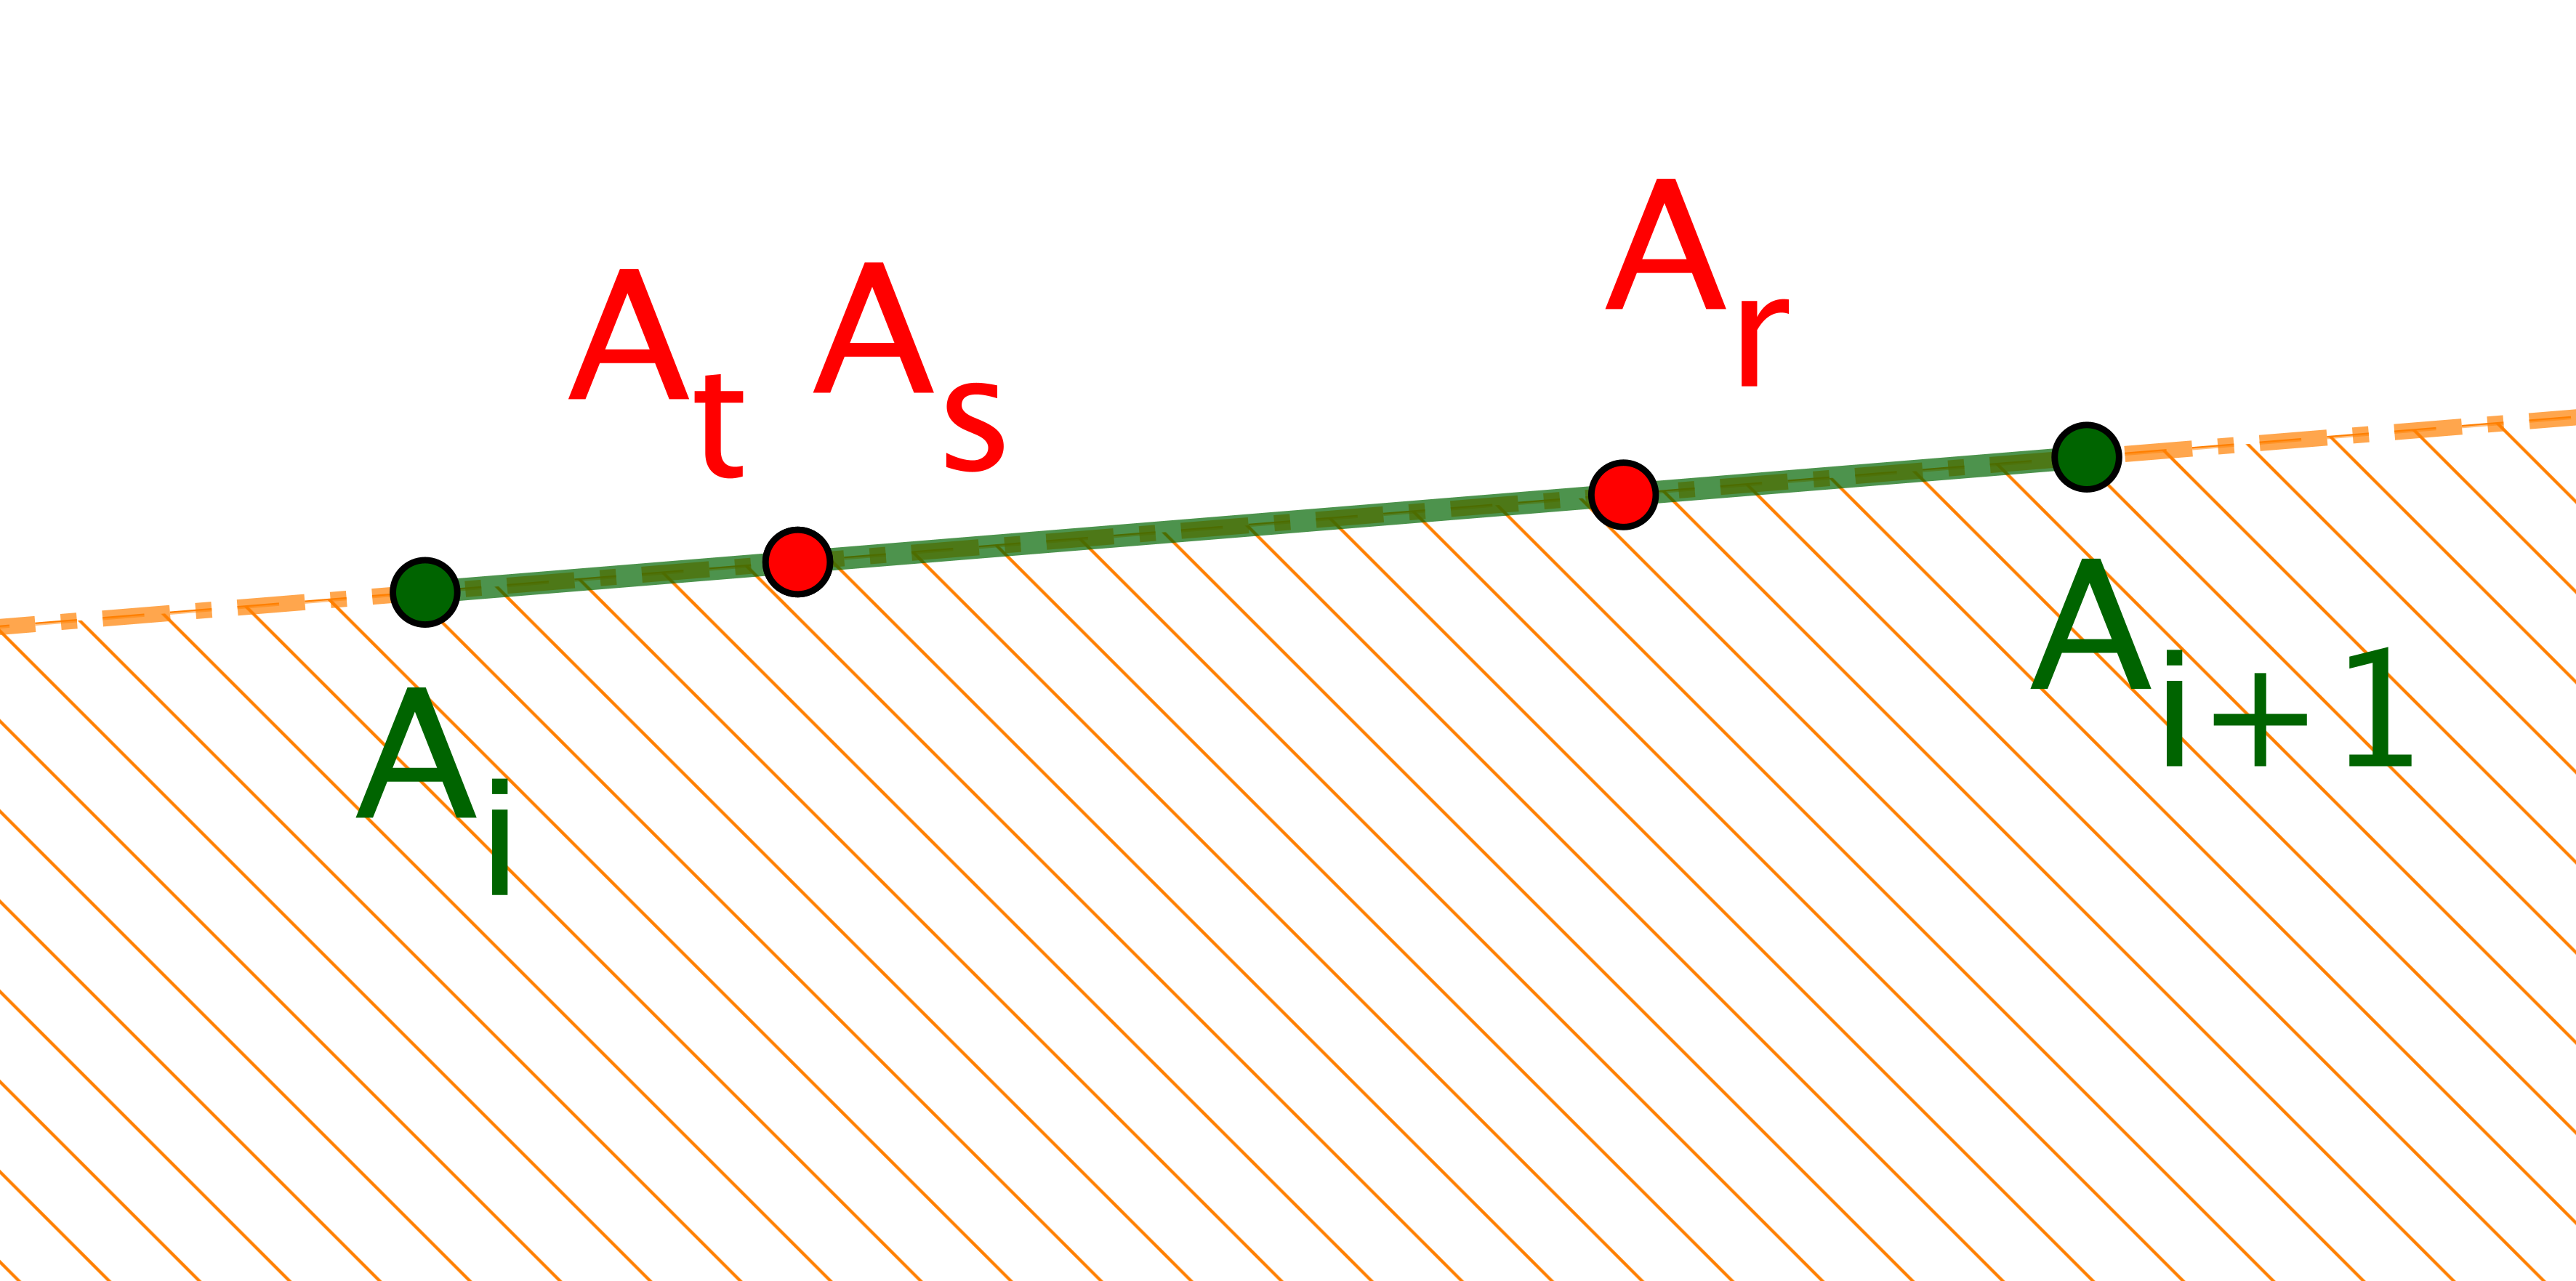
\includegraphics[scale=.4]{content/polygon/at-least-one/max-ngone-1.png}
        	    
        	    \smallskip
                Un cas possible où $\primeit{A}_s = \primeit{A}_t$.
            
                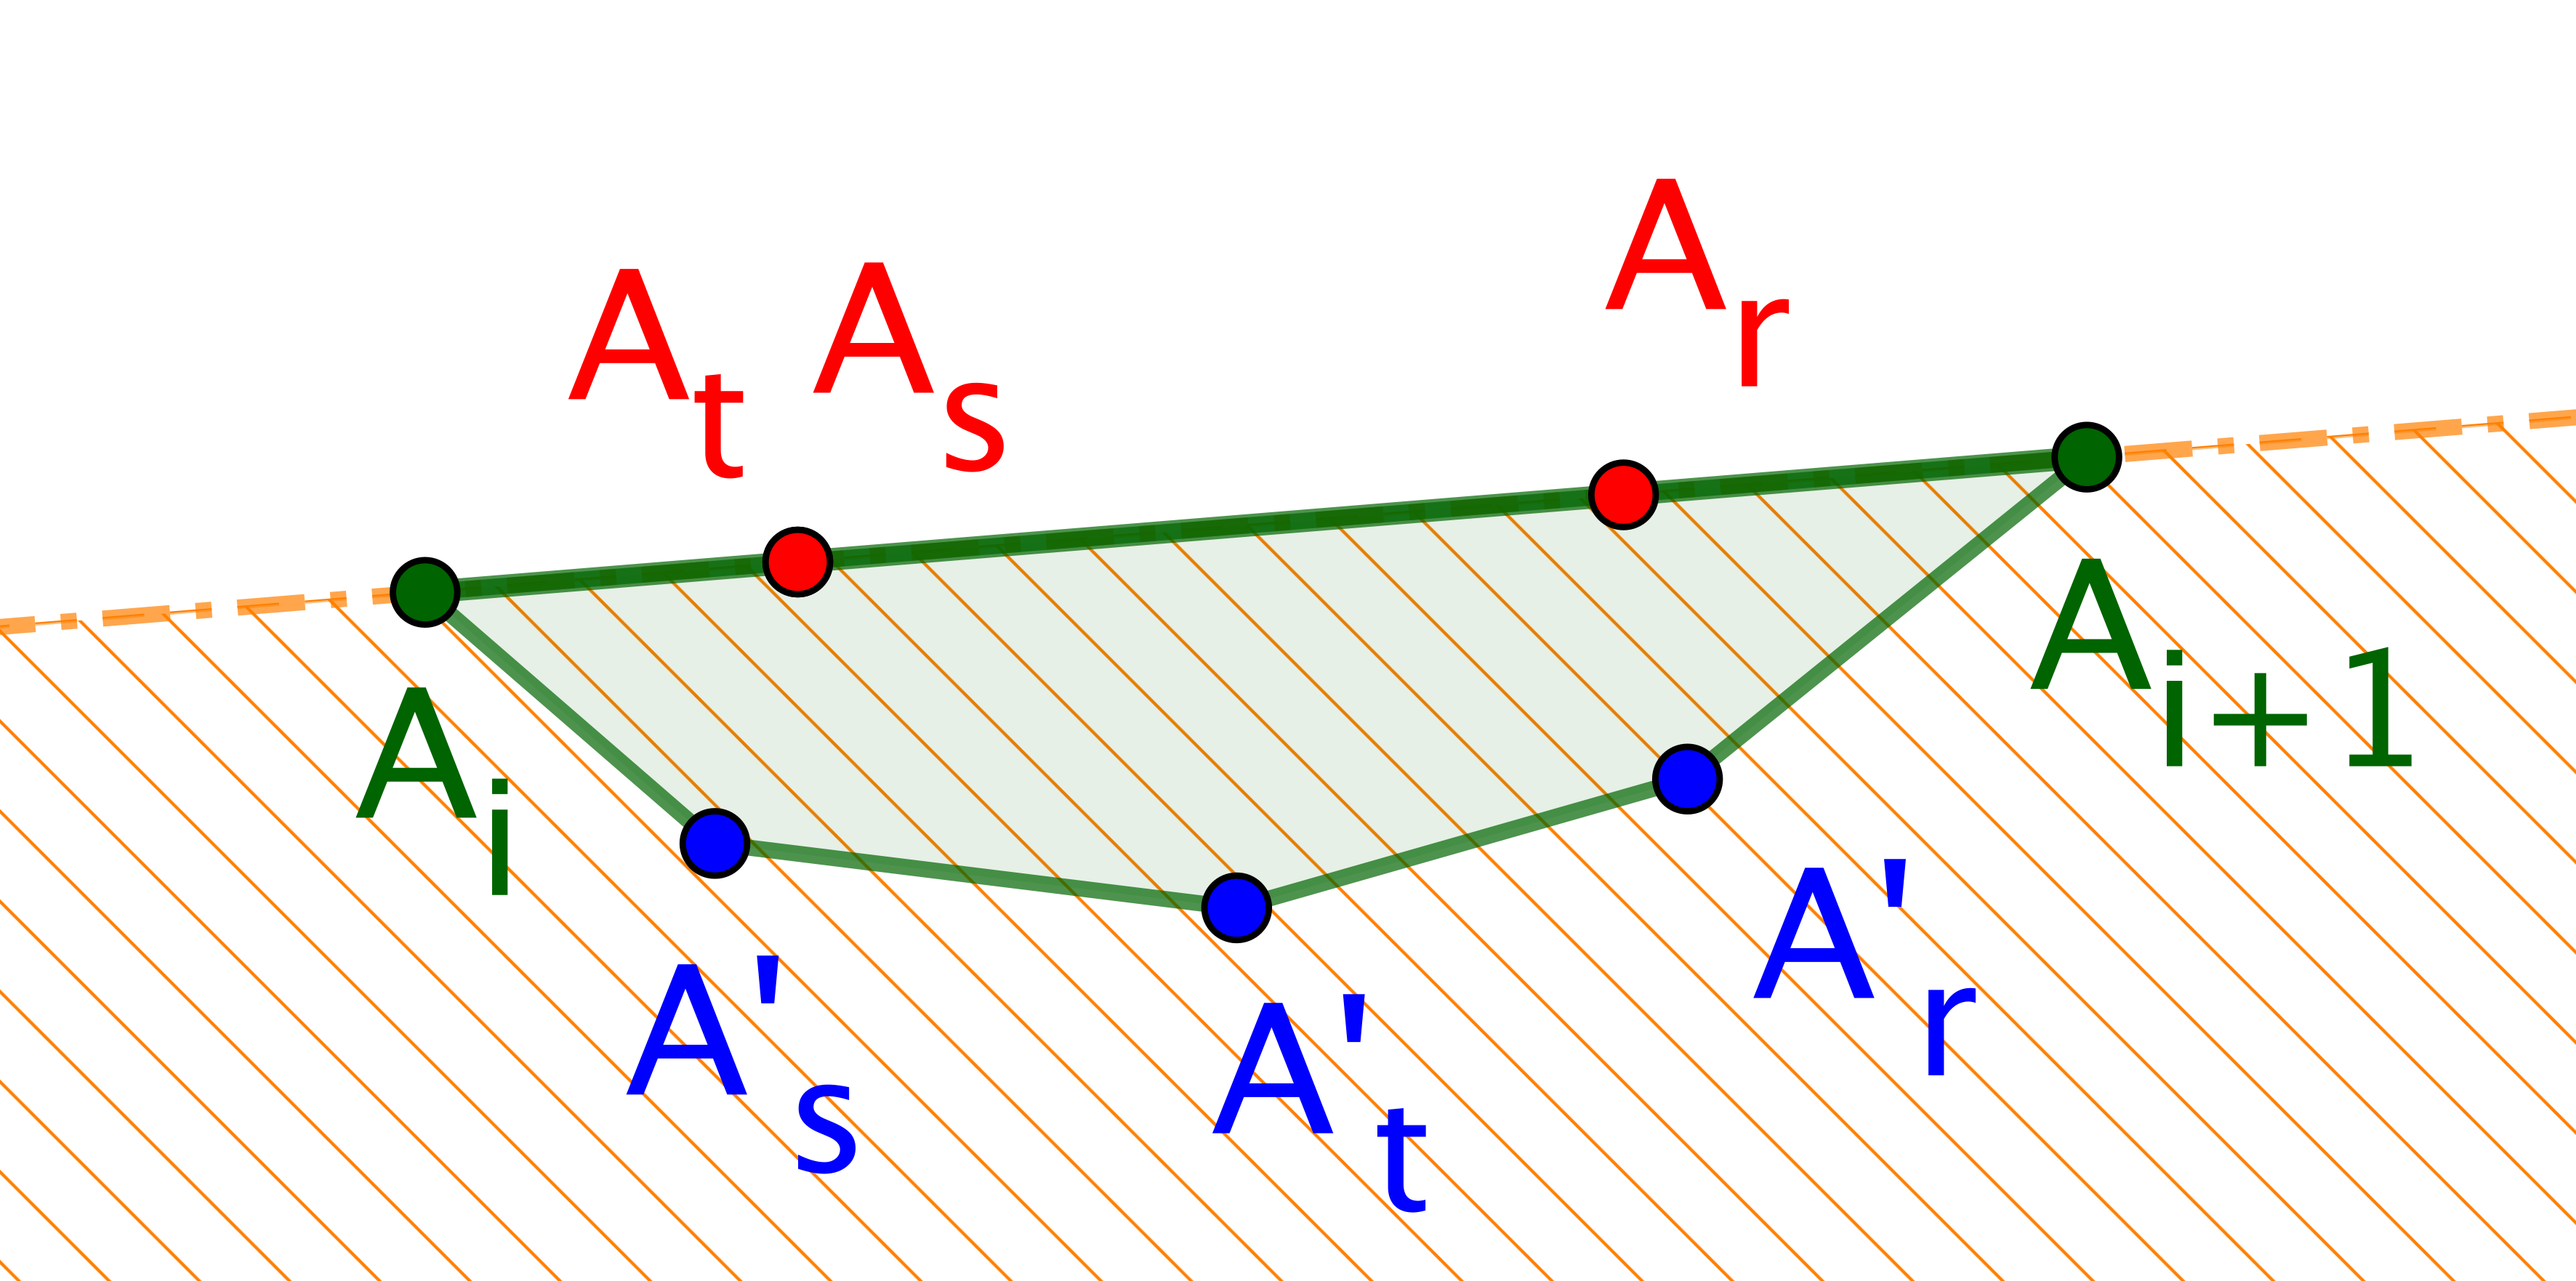
\includegraphics[scale=.4]{content/polygon/at-least-one/max-ngone-2.png}
        	    
        	    \smallskip
                Déformation \focus{convexe possible}.
        \end{multicols}
\end{proof}
